\documentclass[12pt]{article}
\RequirePackage{amsthm,amsmath,amsbsy,amsfonts}
\usepackage{graphicx}
%\usepackage{enumerate}
\usepackage{natbib}
\usepackage{url} % not crucial - just used below for the URL 
\usepackage{placeins}
\usepackage{algorithm}
\usepackage{algpseudocode}
%\pdfminorversion=4
% NOTE: To produce blinded version, replace "0" with "1" below.
\newcommand{\blind}{0}

% DON'T change margins - should be 1 inch all around.
\addtolength{\oddsidemargin}{-.5in}%
\addtolength{\evensidemargin}{-.5in}%
\addtolength{\textwidth}{1in}%
\addtolength{\textheight}{1.3in}%
\addtolength{\topmargin}{-.8in}%


\begin{document}
	
	%\bibliographystyle{natbib}
	
	\def\spacingset#1{\renewcommand{\baselinestretch}%
		{#1}\small\normalsize} \spacingset{1}
	
	
	%%%%%%%%%%%%%%%%%%%%%%%%%%%%%%%%%%%%%%%%%%%%%%%%%%%%%%%%%%%%%%%%%%%%%%%%%%%%%%
	
	\if0\blind
	{
		\title{\bf Baseline Drift Estimation for Time Series Data Using Quantile Trend Filtering}
		\author{Halley Brantley\thanks{
				Department of Statistics, North Carolina State University, Raleigh, NC 27695 (E-mail: hlbrantl@ncsu.edu)} \,
			Joseph Guinness\thanks{
				Department of Biological Statistics and Computational Biology, Cornell University, Ithaca, NY 14853 (E-mail: guinness@cornell.edu )} \,
			and
			%    and
			Eric C. Chi\thanks{Department of Statistics, North Carolina State University, Raleigh, NC 27695 (E-mail: eric$\_$chi@ncsu.edu).}    \\}
		\date{}
		\maketitle
	} \fi
		
	\if1\blind
	{
		\bigskip
		\bigskip
		\bigskip
		\begin{center}
			{\LARGE\bf Title}
		\end{center}
		\medskip
	} \fi
	
	\bigskip
	\begin{abstract}
		We address the problem of estimating smoothly varying baseline trends in time series data using quantile trend filtering. We extend the basic framework to ensure non-crossing while estimating multiple trends simultaneously and implement an alternating direction method of moments (ADMM) algorithm for series that cannot be processed simultaneously. Timing experiments demonstrate the usefulness of our ADMM algorithm even in cases where the series can be processed simultaneously. We also address smoothing parameter selection and propose a modified criteria based on the extended Bayesian Information Criteria. We demonstrate both through simulation studies and an application to low cost air quality sensor data that our model provides better or comparable estimates than existing methods of non-parametric quantile trends and improves signal classification of low-cost air quality sensor output. 
	\end{abstract}
	
	\noindent%
	{\it Keywords:} quantile regression, non-parametric, trend estimation, smoothing splines
	\vfill
	
	\newpage
	\spacingset{1.5} % DON'T change the spacing!
	\section{Introduction}
	\label{sec:intro}
	
	In applications spanning the fields of chemistry \citep{Ning2014}, macroeconomics \citep{yamada2017estimating}, environmental science \citep{brantley2014mobile}, and medical sciences \citep{pettersson2013algorithm, marandi2015qualitative}, scalar time series are observed and assumed to consist of a slowly varying trend and other more rapidly varying components. \cite{Kim2009} addressed the case when the series consisted of just a trend and a random noise component and proposed the use of \textit{$\ell_1$ trend filtering} to estimate trends that piecewise linear or piecewise polynomial. \cite{Tib2014} later demonstrated that empirically the trend filtering estimates adapt to the local level of smoothness better than the more common smoothing splines. In the trend filtering problem, given observations $y(t)$ with $t=1,...,N$, the trend, $\theta(t)$, is estimated by solving the following convex problem.
	\begin{eqnarray}
	\underset{\theta}{\arg\min}\; \frac{1}{2} \lVert y - \theta \rVert_2^2 + \lambda \lVert \mathbf{D}^{(k+1)}\theta \rVert_1,
	\end{eqnarray}
	where $\lambda \geq 0$ is a regularization parameter and the matrix $\mathbf{D}^{(k+1)} \in \mathbb{R}^{(n - k -1) \times n}$ is the discrete difference operator of order $k+1$. To understand the purpose of penalizing $\mathbf{D}^{(k+1)}$ consider the difference operator when $k = 0$.
	\begin{eqnarray}
	\mathbf{D}^{(1)} = \begin{pmatrix}
	-1 & 1 & 0 & \cdots & 0 & 0 \\
	0 & -1 & 1 & \cdots & 0 & 0 \\
	\vdots & & & & & \\
	0 & 0 & 0 & \cdots & -1 & 1 \\
	\end{pmatrix}
	\end{eqnarray}
	Thus, $\lVert \mathbf{D}^{(1)}\theta \rVert_1 = \sum_{i=1}^{n-1} \lvert \theta_i - \theta_{i+1} \rvert$ which is just total variation denoising in one dimension. The penalty incentivizes solutions which are piece-wise constant. For $k \geq 1$, the difference operator $\mathbf{D}^{(k+1)} \in \mathbb{R}^{(n-k-1) \times n}$ is defined recursively as follows
	\begin{eqnarray}
	\mathbf{D}^{(k+1)} & = & \mathbf{D}^{(1)}\mathbf{D}^{(k)}.
	\end{eqnarray}
	By penalizing the $k+1$ fold composition of the discrete difference operator, we obtain solutions which are piecewise polynomials of order $k$. 
	
	Trend filtering provides excellent estimates of trends when the only components of the time series are the trend and random noise (Fig. \ref{fig:trendfilter}). In some applications, however, time series may also include a rapidly varying signal component in addition to the trend and noise, in these cases the trend filtering estimate over-estimates the trend in the places where signal is present (Fig. \ref{fig:trendfilter}).  
	   	
	\begin{figure}
		\centering
		\caption{Examples of trend filtering solutions. The true trend is shown in black, while the estimated trend is shown in red.}
		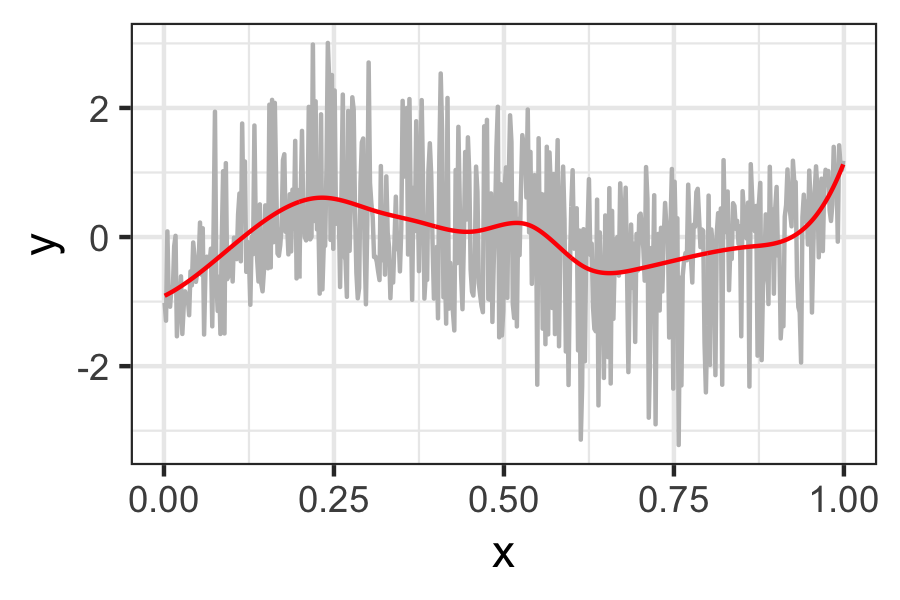
\includegraphics[width = 0.45\linewidth]{Figures/trend_filter_eg1.png}
		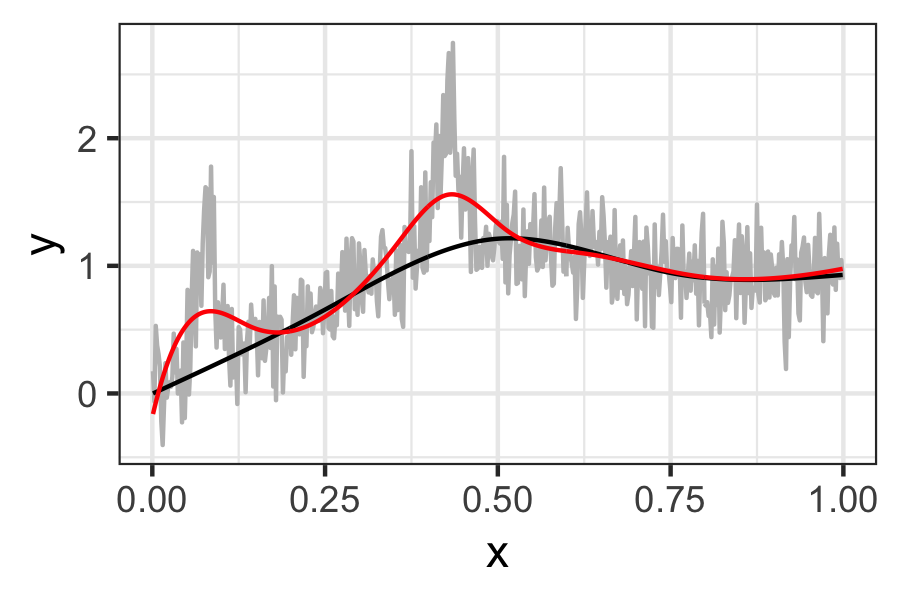
\includegraphics[width = 0.45\linewidth]{Figures/trend_filter_eg2.png}
		\label{fig:trendfilter}
	\end{figure}
	 
	
	One application in which the observed time series consists of a slowly varying baseline, non-negative signal, and rapidly varying noise is the output of low cost air quality sensors. The use of low-cost, portable, air quality sensors has increased dramatically in the last decade. These sensors can provide an un-calibrated measure of a variety of pollutants in near real time, but deriving meaningful information from sensor data remains a challenge \citep{snyder2013changing}. The ``SPod" is a low-cost sensor currently being investigated by researchers at the U.S. Environmental Protection Agency to detect volatile organic compound (VOC) emissions from industrial facilities \citep{thoma2016south}. To reduce cost and power consumption of the SPod, the temperature and relative humidity of the air presented to the photoionization detectors (PIDs) is not controlled and as a result the output signal exhibits a slowly varying baseline drift on the order of minutes to hours. Fig. \ref{fig:raw_spod} provides an example of 3 co-located SPod sensor outputs from near an industrial facility. While all of the sensors response to the pollutant signal, the amount of baseline drift varies from one node to another.
	 
	\begin{figure}[b!]
		\caption{Example of 3 co-located SPod PID sensor readings.}
		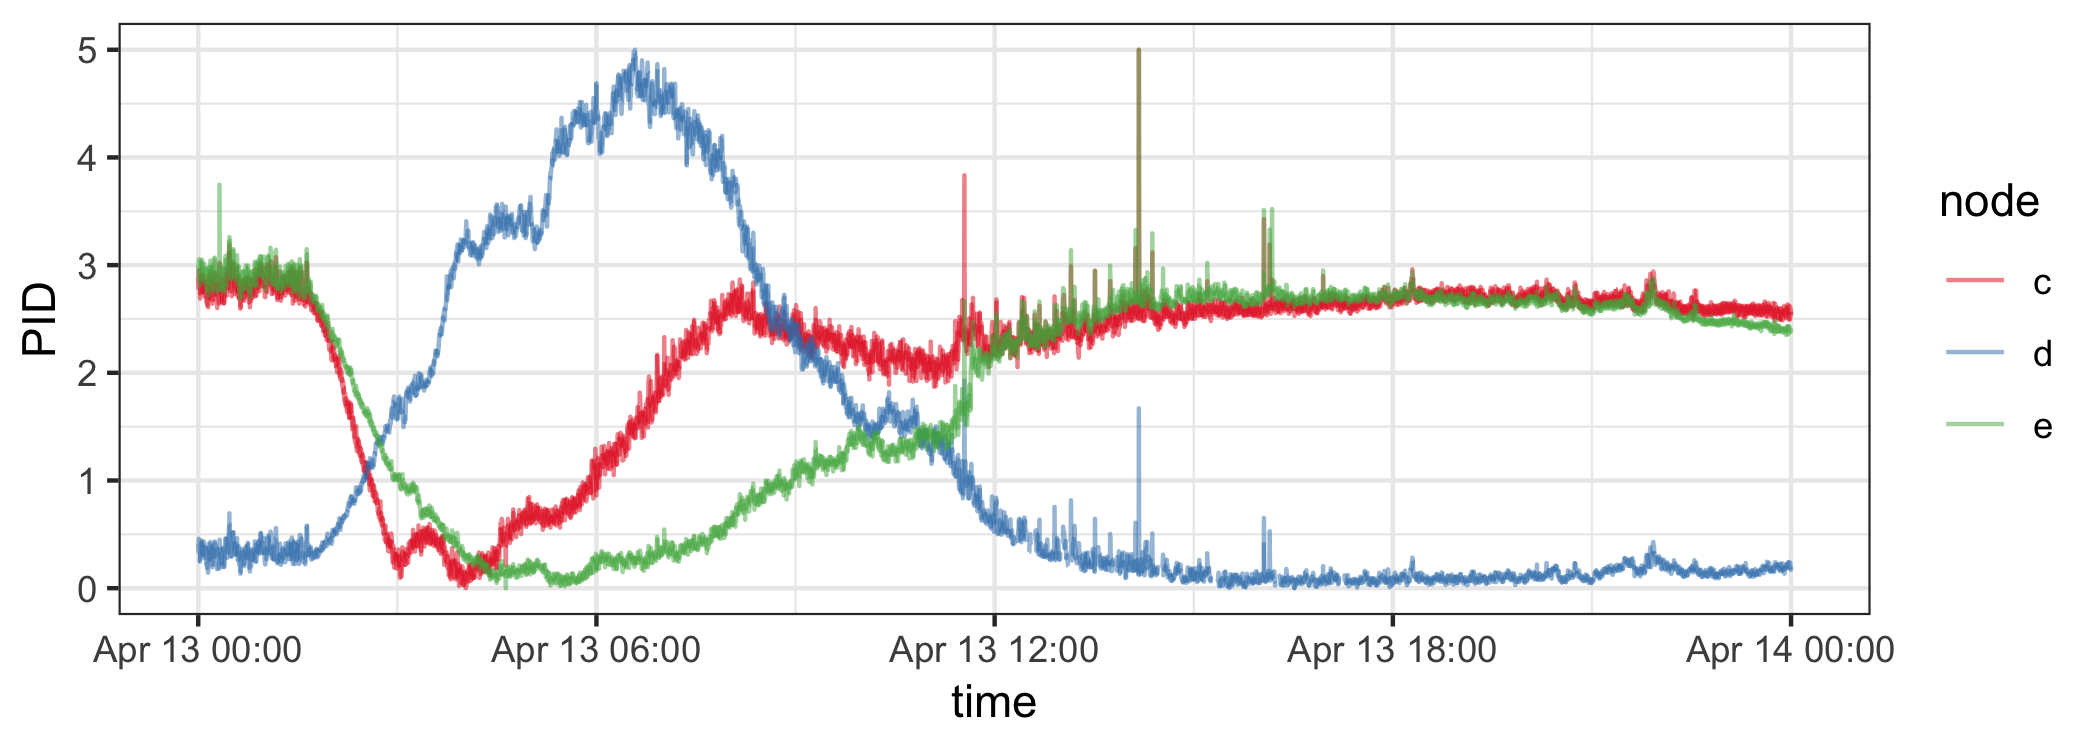
\includegraphics[width = \linewidth]{Figures/uncorrected_data.png}
		\label{fig:raw_spod}
	\end{figure}
   	
	
	In this application, as well as those described in \cite{Ning2014}, \cite{marandi2015qualitative}, and \cite{pettersson2013algorithm}, it is not the mean trend that is desired but rather the baseline trend, which can be thought of as a trend in a low quantile of the data.  \cite{Koenker1978} were the first to propose substituting the squared loss typically used in regression with the check loss function  (Eq. \ref{eq:checkloss}) to estimate a conditional quantile instead of the conditional mean. 
	
	\begin{equation}
	\label{eq:checkloss}
	 \rho_{\tau}(z) = \sum_{i=1}^n z_i(1-\mathbf{I}(z_i<0)).
	\end{equation}
	
	Later, \cite{KoenkerNgPortnoy1994} addressed the issue of estimated quantile curves by combining the check loss penalty with trend filtering penalty with $k = 2$ which produces quantile trends that are piecewise linear. Other approaches to estimating quantile trends have also been proposed. Rather than using the trend filtering $\ell_1$-norm to penalize the discrete differences, \cite{nychka1995nonparametric} used the smoothing spline penalty based on the $\ell_2$-norm solving the optimization problem in Eq. \ref{eq:smoothingspline}. 
	
	\begin{equation*}
	\label{eq:smoothingspline}
	\rho_{\tau}(y - f) + \lambda\int (f''(t))^2 dt, 
 	\end{equation*}
	
	where $f(t)$ is a smooth function of time and $\lambda$ is a tuning parameter that controls the degrees of smoothing. \cite{Oh2011} proposed an algorithm for solving this problem based on approximating the checkloss function with a similar differentiable function. 
	
	\cite{Racine2017} take an entirely different approach to estimating quantile trends. They constrain the response to follow a smooth location scale model of the form $y(t) = a(t) + b(t)\epsilon_i$ and estimate the $\tau$\textsubscript{th} conditional quantile given $t = t_0$ using a kernel estimator and local linear approach. 

	We propose to use the trend filtering penalty combined with the check loss function to produce quantile trends that are piecewise quadratic. The formulation was proposed by \cite{Kim2009} as a possible extension of $\ell_1$-trend filtering but not studied. Moreover we extend the basic framework to ensure non-crossing while modeling multiple quantiles. We also implement a parallel ADMM algorithm for series that are too large to be computed simultaneously and propose a modified criteria for choosing the smoothing parameter. We demonstrate through simulation studies that our proposed model provides better or comparable estimates of non-parametric quantile trends than existing methods and is a more effective method of drift removal for low-cost air quality sensors. 
	

	\section{Methods}
	
	\subsection{Quantile Trend Filtering}
	
	We combine the ideas of quantile regression and trend filtering. For a single quantile level $\tau$ the estimation of the quantile trend filtering model can be posed as the following optimization problem.
	\begin{eqnarray}
	\label{eq:quantile_trend}
	\underset{\theta}{\min}\; \rho_\tau(y - \theta) + \lambda \lVert \mathbf{D}^{(k+1)} \theta \rVert_1,
	\end{eqnarray}
	where $\lambda$ is a non-negative regularization parameter. We address the problem of choosing $\lambda$ in Section \ref{sec:lambda_choice}. As with classic quantile regression, the quantile trend filtering problem is a linear program which can be solved by a number of free or commercial solvers. In many cases, including ours, we are interested in estimating multiple quantiles simultaneously. We also want to ensure that our quantile estimates are valid by enforcing the constraint that if $\tau_2 > \tau_1$ then $Q(\tau_2) \ge Q(\tau_1)$. Given quantiles $\{\tau_1, ..., \tau_J\}$ such that $\tau_1 < \tau_2 < ... < \tau_J$, the optimization problem becomes 
	
	\begin{eqnarray}
	\label{eq:noncross_trend}
	\underset{\theta_1, ..., \theta_J}{\min}\; \sum_{j=1}^J \left [\rho_{\tau_j}(y - \theta_{j}) + 
	\lambda_j \lVert \mathbf{D}^{(k+1)} \theta_j \rVert_1 \right ] \\
	 \text{subject to: }\; \theta_{1}(t) \le \theta_{2}(t) \le ... \le \theta_{J}(t) \text{ for all } t,
	\end{eqnarray}
	
	where $\theta_j \in \mathcal{R}^n$. The additional constraints are linear in the parameters so the non-crossing quantile trends can still be estimated by a number of available solvers. In the rest of this paper we rely on the commercial solver Gurobi \citep{gurobi} and its R package implementation, but it can easily be substituted for a free solver such as the Rglpk package by \cite{rglpk}. The number of parameters to be estimated in this problem is equal to the number of observations multiplied by the number of quantiles of interest. As the size of the data and the number of quantiles grows, all solvers will eventually break. 
	
	\subsection{ADMM for Big Data}
	
	To our knowledge, no one has addressed the problem of finding smooth quantile trends of series that are too large to be processed simultaneously. We propose an alternating direction method of multipliers (ADMM) algorithm for solving large problems in a piecewise fashion. The ADMM algorithm \citep{gabay1975dual, glowinski1975approximation} is fully described by \cite{boyd2011distributed}. We apply the consensus ADMM algorithm to the the quantile regression trend filtering problem given in Eq. \ref{eq:quantile_trend}, by dividing our observed series $y(t)$ with $t = \{1, ..., n\}$ into overlapping windows 
	
	\begin{align*}
	y_1(t) = y(t) & \mbox{~~if~~} 1 \le t \le u_{1}\\
	y_2(t) = y(t) & \mbox{~~if~~} l_{2} \le t \le u_{2} \\
	\cdots & \\
	y_M(t) = y(t) & \mbox{~~if~~} l_{M} \le t \le  n\\
	\end{align*}

	 with boundaries $1 < l_{2} < u_{1} < l_{3} < u_{2} < l_{4} < u_{3} < ...< n$. An illustration is given in Fig. \ref{fig:windows}. Given quantiles $\tau_1 < ... < \tau_J$ to be estimated we define $\theta_{j,m}(t)$ as the value of the $\tau_j$\textsuperscript{th} quantile trend in window $M$ at time point $t$. In order to write out the constraint that the overlapping sections must be equal we define a consensus variable
	 
	 \begin{align*}
		 \bar{\theta}_{j,m} =&  g(\theta_{j, m-1}, \theta_{j,m}, \theta_{j,m+1}) \\
		 =& \begin{cases} 
			 \frac{\theta_{j,m-1}(t)+\theta_{j,m}(t)}{2} & \mbox{if~~} l_{m} \le t \le u_{m-1}  \\
			 \theta_{j,m}(t) & \mbox{if~~} u_{m-1} \le t \le l_{m+1}  \\
			 \frac{\theta_{j,m}(t)+\theta_{j,m+1}(t)}{2} & \mbox{if~~} l_{m+1} \le t \le u_{m}  
			 \end{cases},
	\end{align*}
	defining $\theta_{j,M+1} = \theta_{j,M}$ and $\theta_{j,0} = \theta_{j,1}$. Our windowed quantile trend optimization problem can then be written as 
	 \begin{align*}
		 \label{eq:quantile_windows}
		 &\sum_{m=1}^M\underset{\theta_{1,m}, ..., \theta_{J,m}}{\min}\; \sum_{j=1}^J \left [\rho_{\tau_j}(y_m - \theta_{j,m}) + 
		 \lambda_j \lVert \mathbf{D}^{(k+1)} \theta_{j,m} \rVert_1 \right ] \\
		 &\text{subject to: }\; \\
		 &\qquad \theta_{1,m}(t) \le \theta_{2,m}(t) \le ... \le \theta_{J,m}(t) \text{ for all } m,t \\
		 &\qquad \theta_{j,m}(t) = \bar{\theta}_{j,m}(t) \text{ for all } j, m, t
	 \end{align*}
	 Defining Lagrange multipliers $\omega_{j,m}$, and penalty parameter $\gamma > 0$ we can write the augmented Lagrangian for finding the trends in window $m$:
	 \begin{equation*}
	 \mathcal{L}(\theta_{j,m}, \bar{\theta}_{j,m}, \omega_{j,m}) = \sum_{j=1}^J\rho_{\tau_j}(y_m - \theta_{j,m})+\lambda \lVert \mathbf{D}^{(k+1)}\theta_{j,m}\rVert_1 +  \omega_{j,m}^T(\theta_{j,m} - \bar{\theta}_{j,m}) + 
	 \frac{\gamma}{2}||\theta_{j,m} - \bar{\theta}_{j,m}||_2^2
	 \end{equation*}
	 We then estimate the trend separately in each window, which can be done in parallel, while constraining the overlapping pieces of the trends to be equal as outlined in algorithm 1. 
	 
	\begin{figure}[!h] 
		\centering
		\caption{Window boundaries and trends fit separately in each window.}
		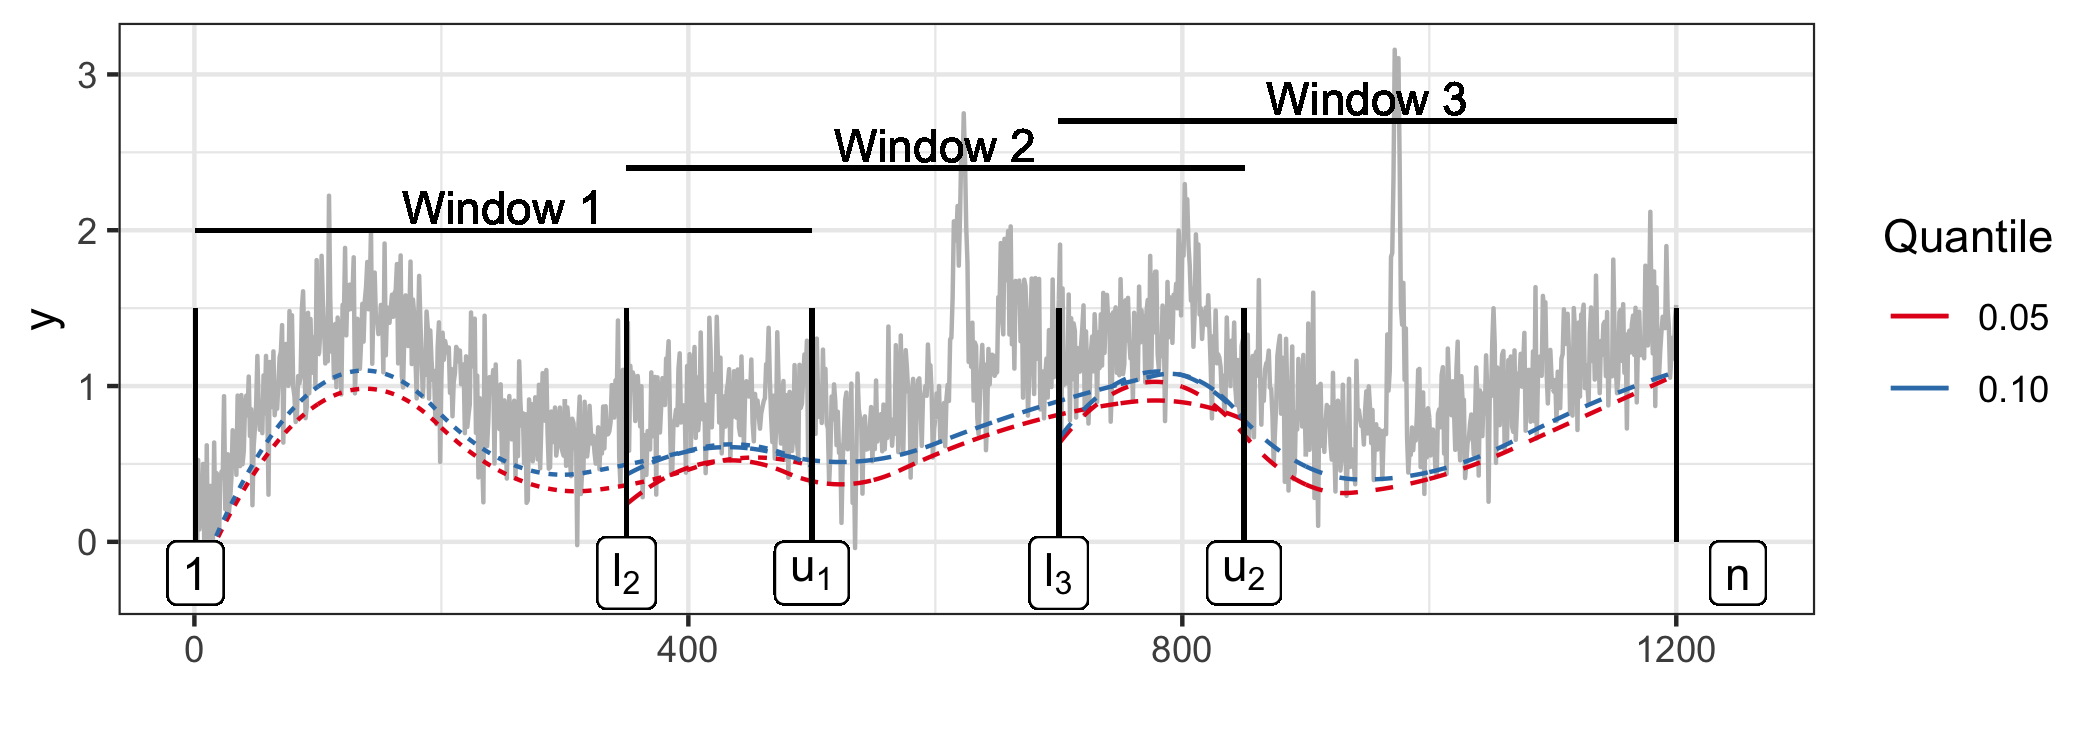
\includegraphics[width = 0.8\linewidth]{Figures/overlapping_windows.png}
		\label{fig:windows}
	\end{figure}

	\begin{algorithm}
		\caption{ADMM algorithm for quantile trend filtering with windows}\label{euclid}
		\begin{algorithmic}		
			\State Define $D = D^{(k+1)}$. 
			\State \textbf{initialize:} \\
				 $\theta_{j,m}^{(0)} = \arg \min \sum_{j=1}^J\rho_{\tau_j}(y_m - \theta_{j,m})+\lambda \lVert D\theta_{j,m}\rVert_1$ subject to $\theta_{1,m}(t) < ...<\theta_{J,m}(t)$ for all $t$. \\		
			 	 $\omega_{j,m}^{(0)} = \mathbf{0}$	
			\Repeat{}
			\State  		
			$\bar{\theta}_{j,m}^{(q)} = g(\theta_{j, m-1}^{(q-1)}, \theta_{j,m}^{(q-1)}, \theta_{j,m+1}^{(q-1)})$
			\State 
			$\omega_{j,m}^{(q)} = \omega_{j,m}^{(q-1)} + \gamma(\theta_{j,m}^{(q-1)} - \bar{\theta}_{j,m}^{(q)})$	
			\State
				$\theta_{j,m}^{(q)} = \arg\min \mathcal{L}(\theta_{j,m}, \bar{\theta}_{j,m}^{(q-1)}, \omega_{j,m}^{(q-1)})$			
			 subject to $\theta_{1,m}(t) < ...<\theta_{J,m}(t)$ for all $t$.
			\Until {convergence}
			\State \textbf{return} Non-overlapping sequence of $\bar{\theta}_{j,m}^{(q)}$ for all $j$, $m$.
			
		\end{algorithmic}
	\end{algorithm}

	We measure convergence use the stopping criteria described by \cite{boyd2011distributed}. The criteria are based on the primal and dual residuals which represent the residuals for the primal and dual feasibility, respectively. The primal residual, 
	\begin{equation}
	r_p^{(q)} = \sqrt{\sum_{m=1}^M\sum_{j=1}^J\lVert\theta_{j,m}^{(q)} - \bar{\theta}_{j,m}^{(q)}\rVert_2^2},
	\end{equation}
	represents the difference between the trend values in the windows and the consensus trend value while the dual residual,
	\begin{equation*}
	r_d^{(q)} = \gamma\sqrt{\sum_{m=1}^M \sum_{j=1}^J\lVert\bar{\theta}_{j,m}^{(q)} - \bar{\theta}_{j,m}^{(q-1)}\rVert_2^2},
	\end{equation*}
	represents the change in the consensus variable from one iterate to the next. The algorithm is stopped when 
	\begin{align}
		&r_p^{(q)} < \epsilon_{abs}\sqrt{nJ} + \epsilon_{rel}\underset{m}{\max}\left[\max 
		\left(\sqrt{\sum_{j=1}^J \lVert\theta_{j,m}^{(q)}\rVert_2^2}, \sqrt{\sum_{j=1}^J \lVert \bar{\theta}_{j,m}^{(q)} \rVert_2^2} \right )\right]\\
		&r_d^{(q)} < \epsilon_{abs}\sqrt{nJ} + \epsilon_{rel}\sqrt{\sum_{m=1}^M\sum_{j=1}^J\lVert \omega_{j,m}^{(q)}\rVert_2^2}
	\end{align}
	

	
	\begin{figure}
		\centering
		\caption{Trend fit with our ADMM algorithm with 3 windows which converged in 7 iterations compared to trend from simultaneous fit.}
		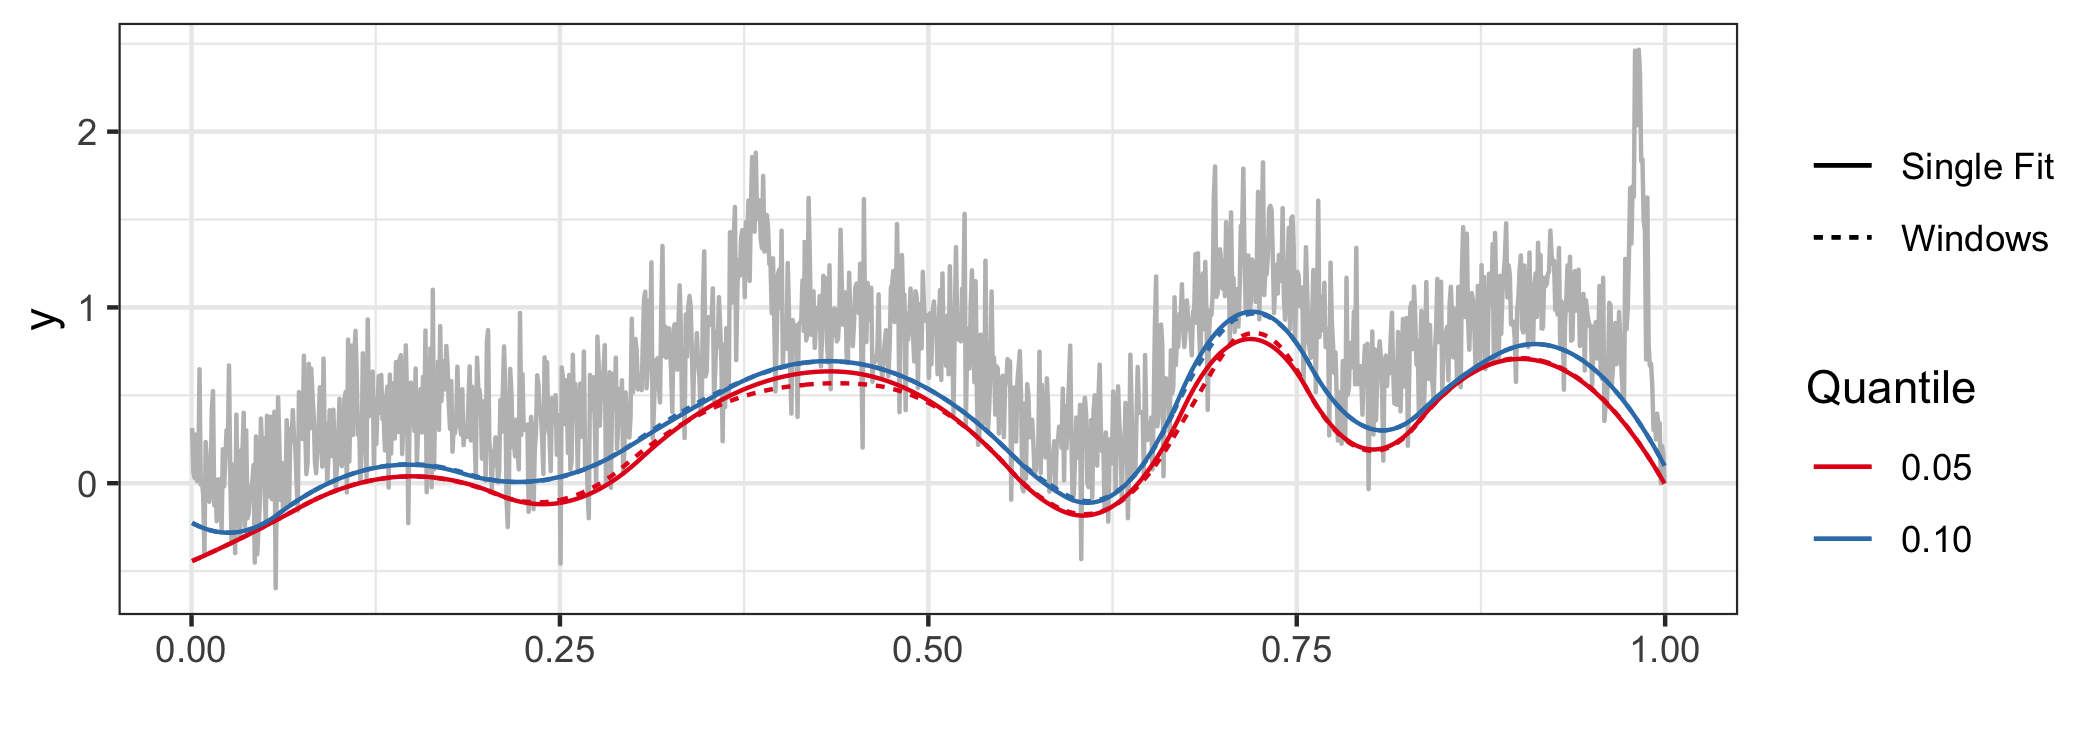
\includegraphics[width = 0.8\linewidth]{Figures/admm_windows.png}
	\end{figure}

	Timing experiments illustrate the advantages of using our ADMM algorithm even on datasets where solving the problem simultaneously is possible. For each data size, $n$, 25 datasets were simulated using the peaks simulation design described below and trends for three quantiles were fit simultaneously: 0.05, 0.1, and 0.15 using a $\lambda = n/5$. We use from one to four windows for each data size with an overlap of 500. The windows algorithm was run until the stopping criteria were met using $\epsilon_{abs} = 0.01$ and $\epsilon_{rel} = 0.001$. As is shown in Fig. \ref{fig:timing}, using 4 windows instead of one on data sizes of 55000 provides a factor of 3 decrease in computation time. The timing experiments were conducted on   
	
	\begin{figure}[!h] 
		\centering
		\caption{Timing experiments comparing quantile trend filtering with varying numbers of windows by data size.}
		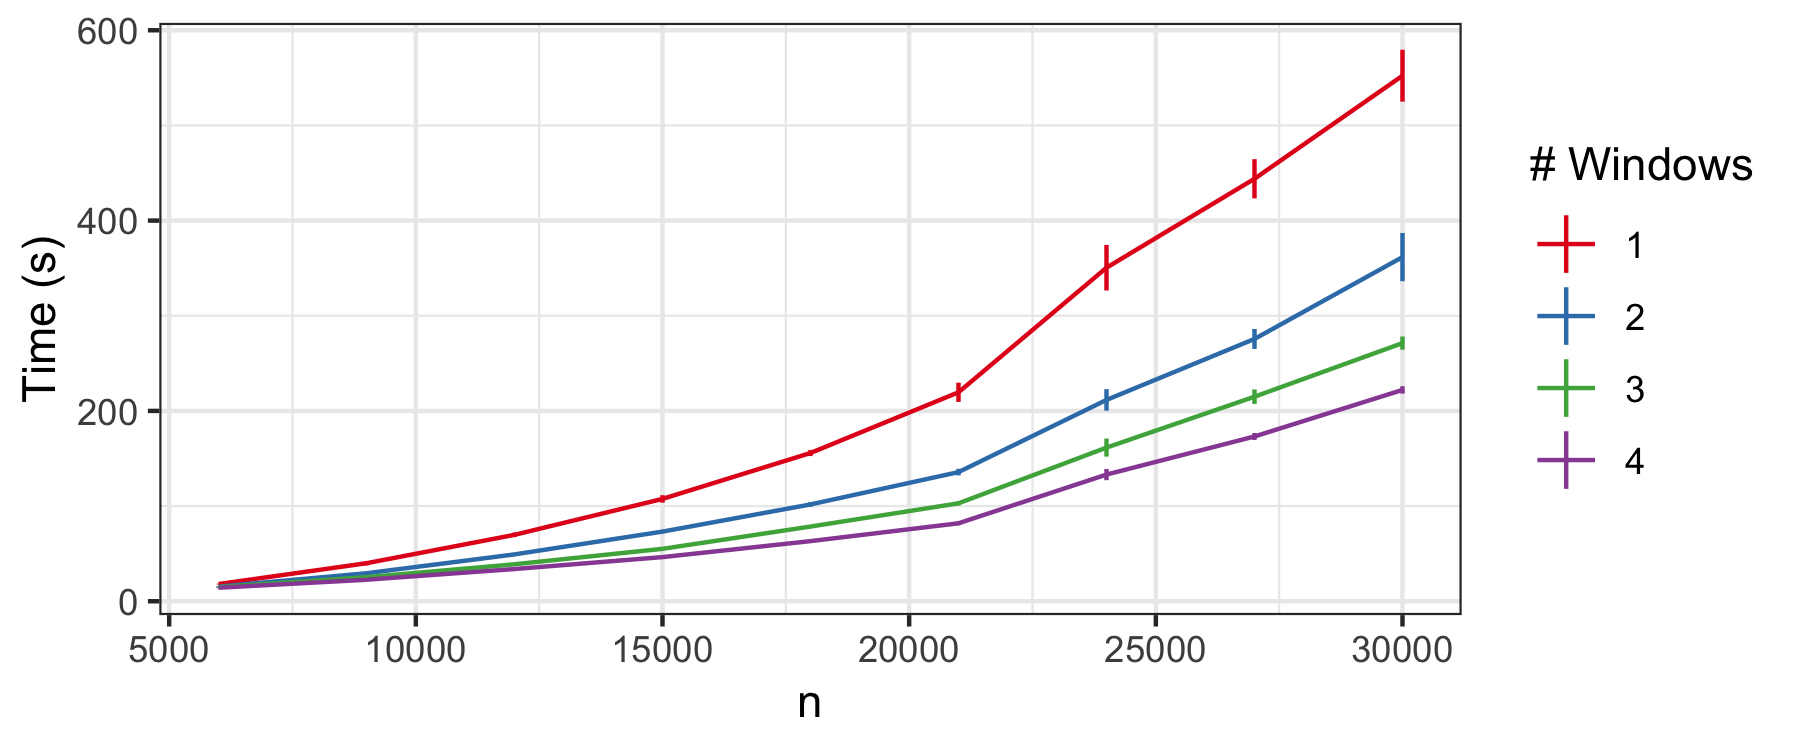
\includegraphics[width = 0.7\linewidth]{Figures/Fig_timing_experiment.png}
		\label{fig:timing}
	\end{figure}

	\subsection{Regularization Parameter Choice}
	\label{sec:lambda_choice}
	An important problem in trend estimation is the choice of regularization parameter or degree of smoothness. Our method can easily handle missing data by defining the check loss function to output 0 for missing values. This allows us to leave out validation observations that can be used to select the tuning parameter $\lambda$. However, the use of an information criteria metric can result in a better choice of regularization parameter than the validation method.  \cite{KoenkerNgPortnoy1994} addressed the choice of regularization parameter by proposing the Schwarz criterion for the selection of $\lambda$
	\begin{equation}
	\label{eq:SIC}
	\mbox{SIC}(p_{\lambda}) = \log\left[\frac{1}{n}\rho_{\tau}(y - \theta)\right] + \frac{1}{2n}p_{\lambda}\log n.
	\end{equation}
	where $p_{\lambda} = \sum_t I(y(t) = \widehat{\theta}(t))$ is the number of interpolated points, which can be thought of as active knots. The SIC is based on the traditional Bayesian Information Criterion (BIC) which is given by 
	\begin{equation}
	\mbox{BIC}(s) = -2\log(L\{\hat{\theta}\}) + \nu\log n 
	\end{equation}	
	where $L$ is the likelihood function and $\nu$ is the number of non-zero components in $\hat{\theta}$. If we take the approach used in Bayesian quantile regression \citep{yu2001bayesian}, and assume that minimizing the checkloss function corresponds to maximizing the asymmetric Laplace likelihood, \begin{equation}
	L(y|\theta) = \left(\frac{\tau^n(1-\tau)}{\sigma}\right)^n\exp\left\{-\sum_t\rho_\tau\left(\frac{y(t) - \theta(t)}{\sigma}\right)\right\},
	\end{equation} 
	we can compute the BIC as 
	\begin{equation}
	\mbox{BIC}(df) = 2\frac{1}{\sigma}\rho_{\tau}(y-\hat{\theta}) + \mbox{df}\log n
	\end{equation} 
	where $df$ is the number of non-zero elements of $D^{(k+1)}\hat{\theta}$. We can choose any $\sigma>0$ and have found empirically that $\sigma =  \frac{1-|1-2\tau|}{2}$ produces stable estimates. 
	
	Another criteria, the extended Bayesian Information Criteria (eBIC), specifically designed for large parameter spaces was proposed by \cite{chen2008}. 
	\begin{equation}
	\label{eq:eBIC}
	\mbox{eBIC}_{\gamma}(s) = -2\log(L\{\hat{\theta}\}) + \nu\log n  + 2\gamma\log{P \choose \nu},~~\gamma \in [0,1]
	\end{equation}
	where $P$ is the total number of possible parameters and $\nu$ is the number of non-zero parameters included in given model. We used this criteria with $\gamma = 1$, and $P=n-k-1$. We use a single dataset from our simulation study to illustrate the difference between the scaled, unscaled ($\sigma = 1$) and scaled extended BIC criteria in Fig. \ref{fig:BIC}. 
	
	\begin{figure}[h!]
		\caption{(Left) Degrees of freedom (number of non-zero elements of $D\theta$) by $\log(\lambda)$. (Middle) Estimated 10th quantile trend with regularization parameter chosen using various criterion. (Right) Criterion values by $\log(\lambda)$ vertical lines indicate locations of minima.} 
		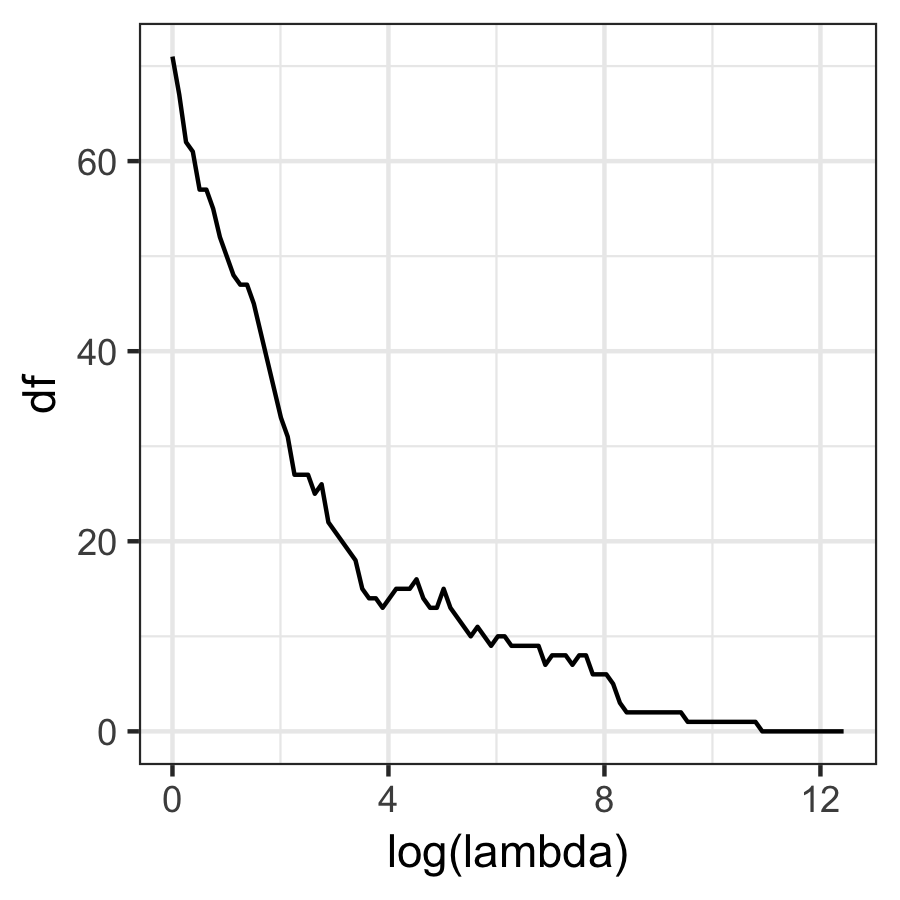
\includegraphics[width = 0.25\linewidth]{Figures/df_by_lambda.png}
		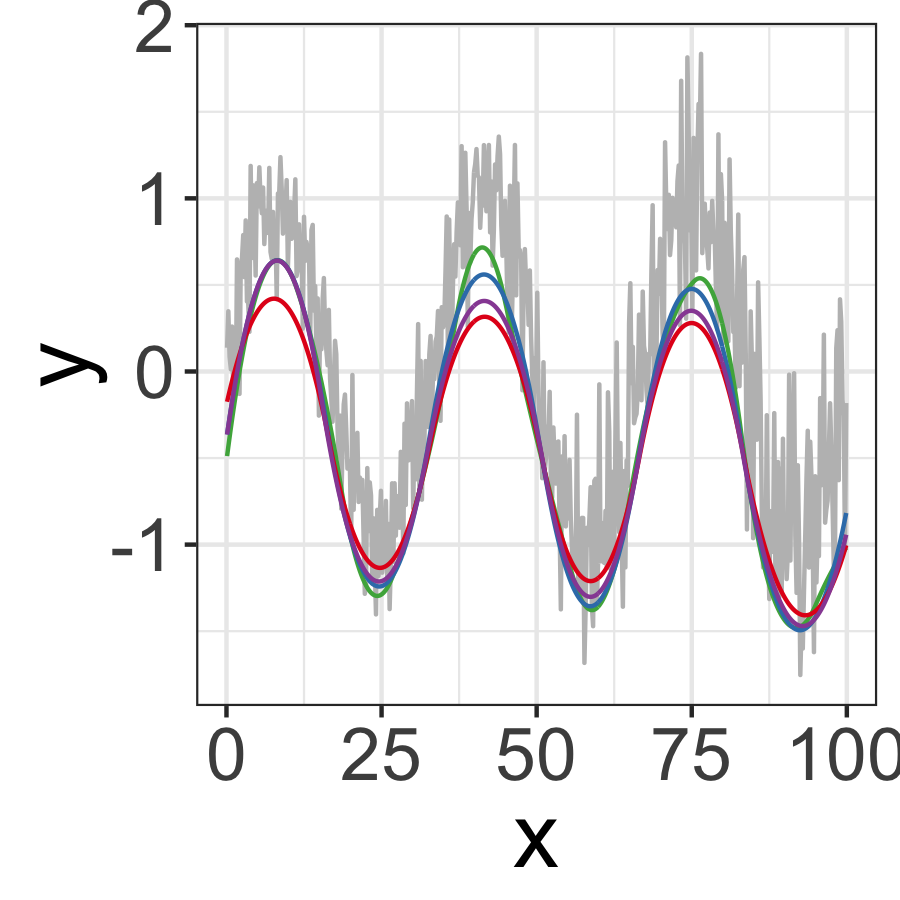
\includegraphics[width = 0.25\linewidth]{Figures/BIC_data.png}
		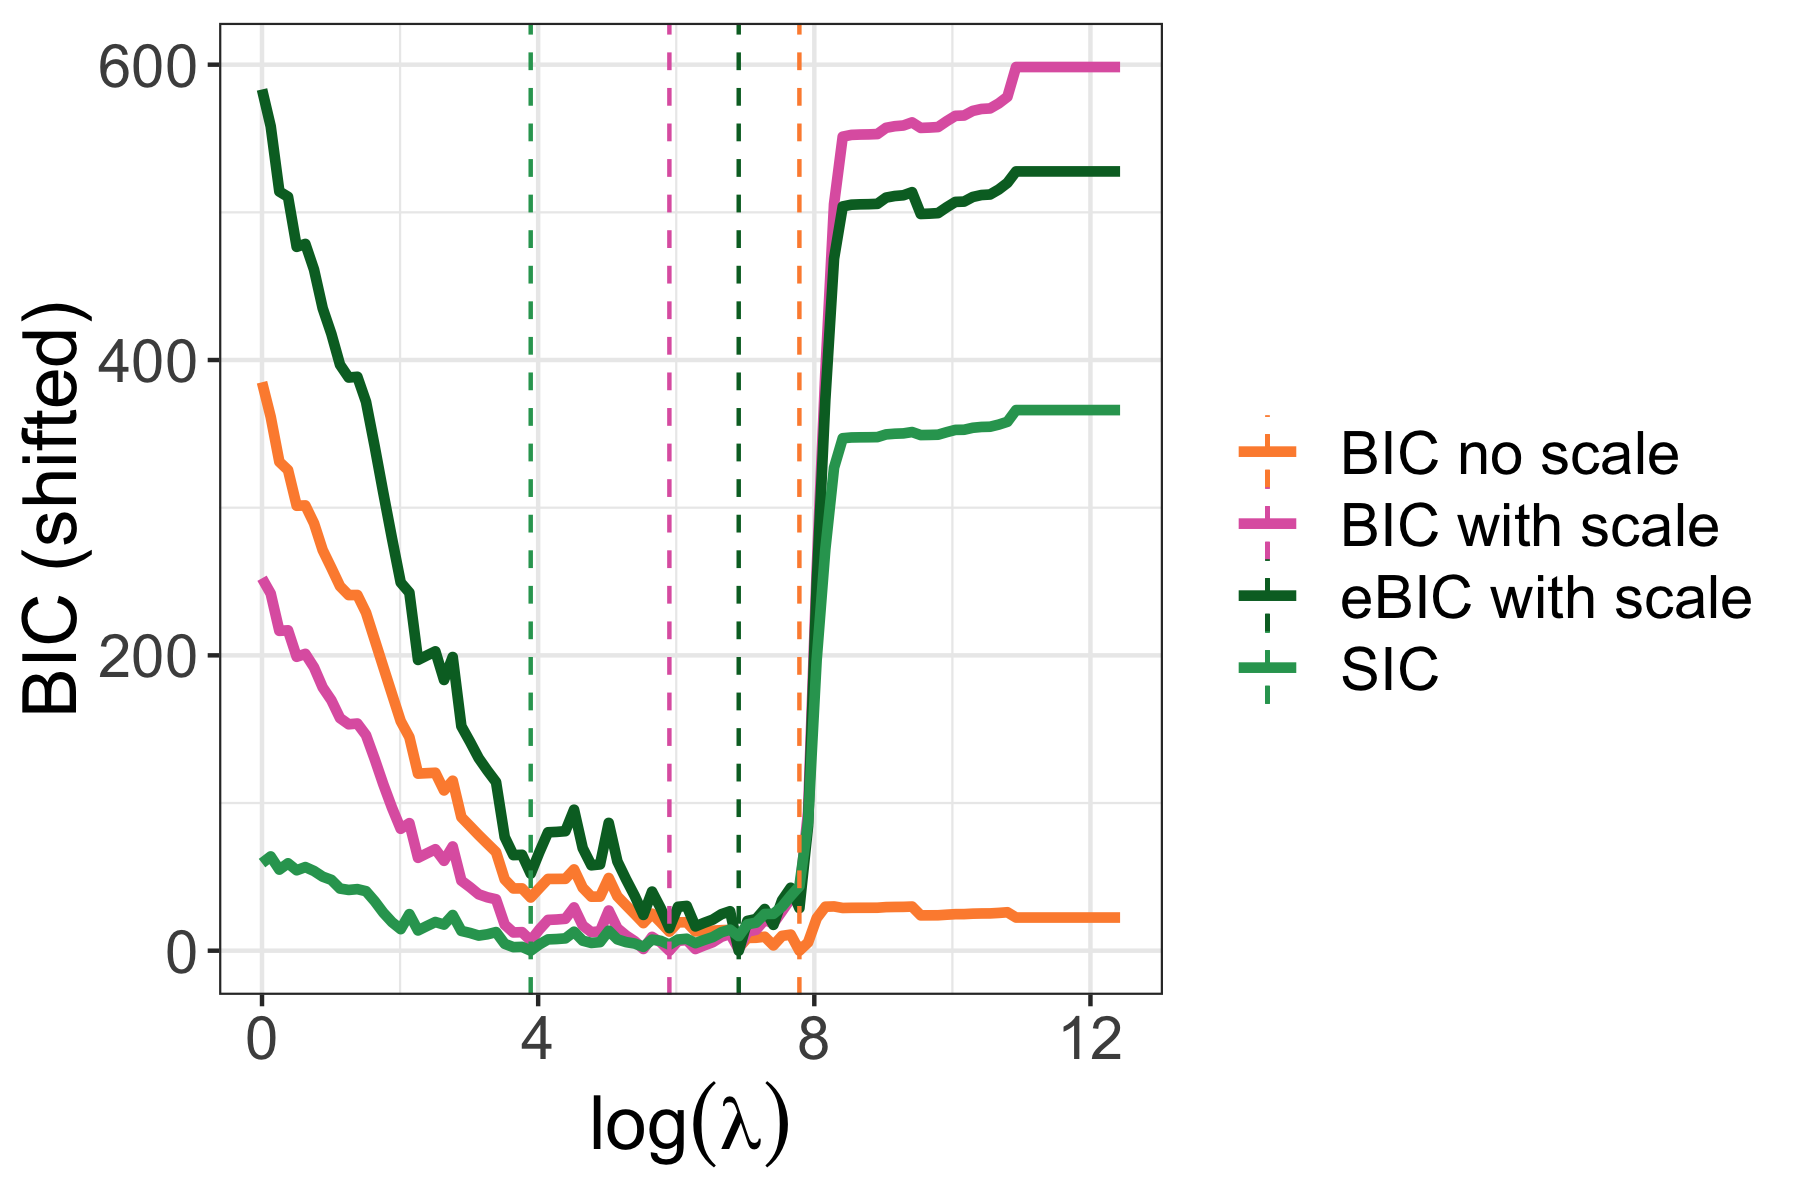
\includegraphics[width = 0.5\linewidth]{Figures/BIC_by_lambda.png} 
		\label{fig:BIC}
	\end{figure}

	\section{Simulation Studies}
	
	We conduct two simulation studies to compare the performance of our quantile trend filtering method and regularization parameter selection criteria with previously published methods. The first study compares the method's ability to estimate quantiles when the only components of the observed series are a smooth trend and a random component. The second study is based on our application and compares the method's ability to estimate baseline trends and enable peak detection when the time series contains a non-negative signal component in addition to the trend and random component. 
	
	We compare the performance of our quantile trend filtering method with three previously published methods: \texttt{npqw} which is the quantile-ll method described in \cite{Racine2017}, code was obtained from the author; \texttt{qsreg} in the \texttt{fields} R package and described in \cite{Oh2011, nychka1995nonparametric}; \texttt{rqss} available in the \texttt{quantreg} package and described in \cite{KoenkerNgPortnoy1994}.  The regularization parameter $\lambda$ for the \texttt{rqss} method is chosen using a grid search and minimizing the SIC criteria as described in \cite{KoenkerNgPortnoy1994}, the regularization parameter for \texttt{qsreg} was chosen using generalized cross-validation based on the quantile criterion \cite{Oh2011}. 
	
	We also compare three criteria for choosing the smoothing parameter with our quantile trend filtering method with a single window: \texttt{detrendr\_SIC} $\lambda$ chosen using SIC (Eq. \ref{eq:SIC}) \citep{KoenkerNgPortnoy1994}; \texttt{detrendr\_valid}: $\lambda$ is chosen by leaving out every 5th observation as a validation data set and minimizing the check loss function evaluated at the validation data; \texttt{detrendr\_eBIC}:  the proposed scaled eBIC criteria (Eq. \ref{eq:eBIC}). 
	
	 
	\subsection{Estimating Quantiles}
	\begin{figure}
		\caption{Simulated data with true quantile trends.}	
		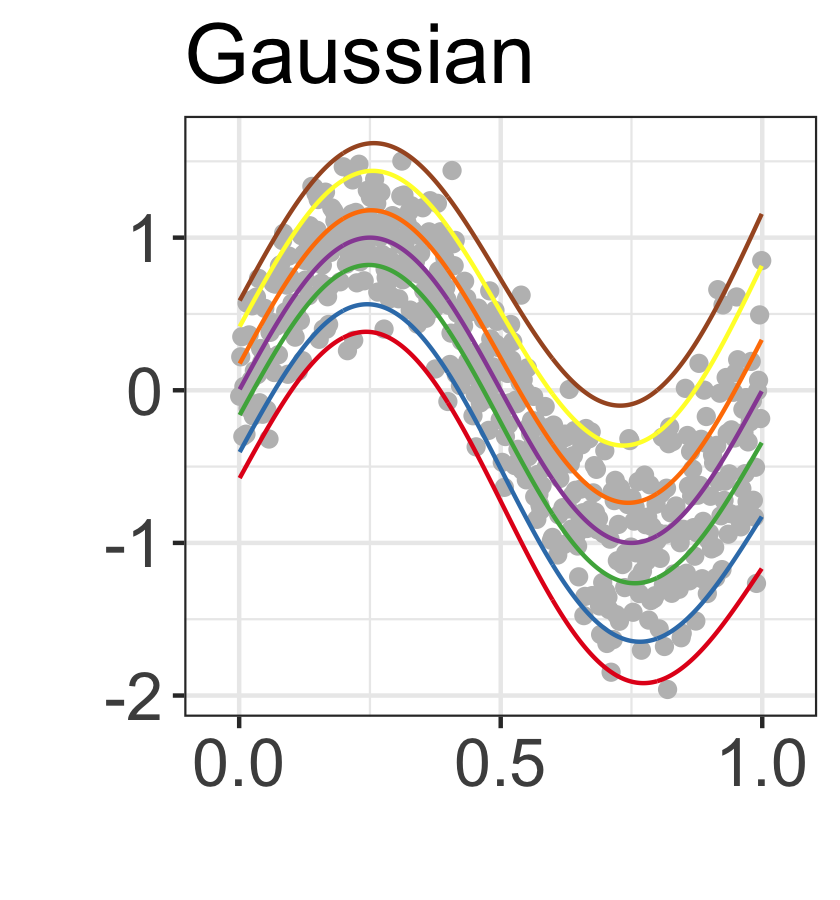
\includegraphics[width=.28\linewidth]{Figures/gaus.png}
		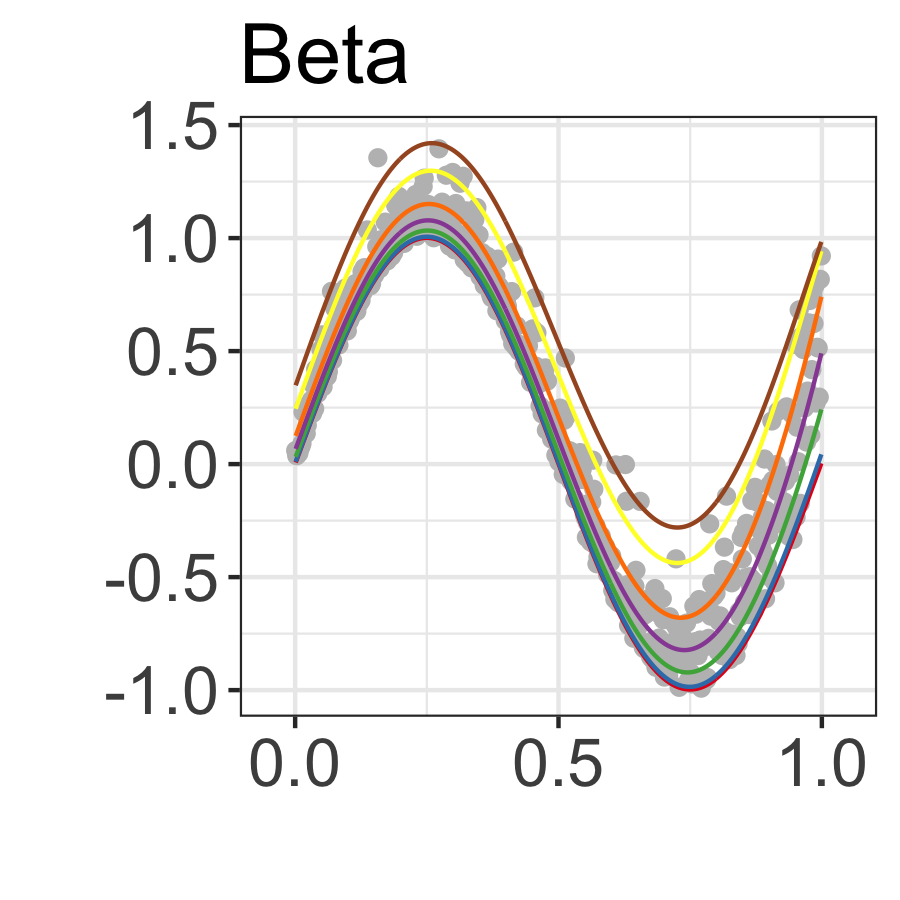
\includegraphics[width=.3\linewidth]{Figures/shapebeta.png}
		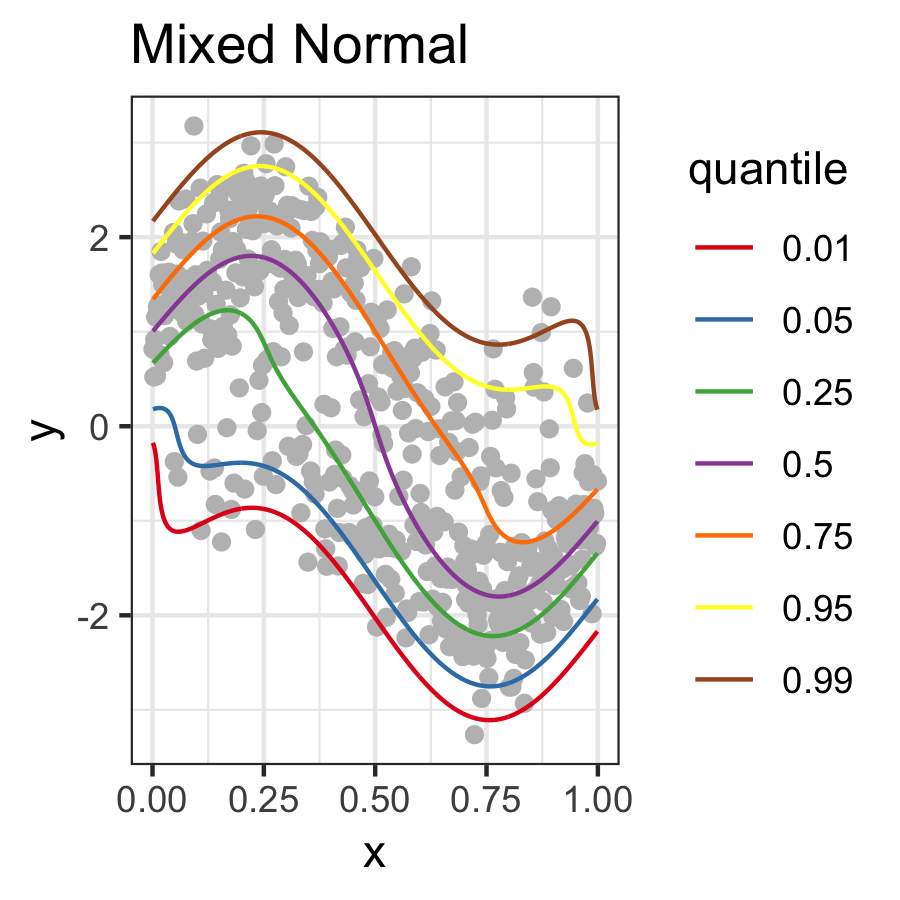
\includegraphics[width=.45\linewidth]{Figures/mixednorm.png}
	\end{figure}

	To compare performance in estimating quantile trends, three simulation designs from \cite{Racine2017} were considered. For all designs $t = 1, ..., n$,  $x(t) = t/n$, and the response $y$ was generated as 
	$$y(t) = sin(2\pi x(t)) + \epsilon(x(t))$$
	The three error distributions considered were 
	\begin{itemize}
		\item Gaussian: $\epsilon(x(t)) \sim N\left(0, \left(\frac{1+x(t)^2}{4}\right)^2\right)$
		\item Beta: $\epsilon(x(t)) \sim Beta(1, 11-10x(t))$
		\item Mixed normal: $\epsilon(x(t))$ is simulated from a mixture of $N(-1,1)$ and  $N(1,1)$ with mixing probability $x(t)$.
	\end{itemize}
	
	One hundred datasets were generated of sizes 300, 500 and 1000. For each method quantile trends were estimated for $\tau = \{0.05, 0.25, 0.5, 0.75, 0.95\}$. Only our detrend methods guarantee non-crossing quantiles. For each quantile trend and method the root mean squared error was calculated as $\mbox{RMSE} = \sqrt{\frac{1}{n}\sum_t (\hat{q}_{\tau}(t) - q_\tau(t))^2}$. The mean RMSE $\pm$ twice the standard error for each method, quantile level and sample size is shown in Figure \ref{fig:quantile_mse}. 	In all three designs the proposed detrend methods are either better than or comparable to existing methods. Overall the \texttt{detrend\_eBIC} performs best, and especially in the mixed normal design our methods have lower RMSEs for the 5\textsuperscript{th} and 95\textsubscript{th} quantiles. The \texttt{npqw} method performs particularly poorly in the mixed normal design due to the fact that it assumes the data comes from a scale-location model which is violated in this case. 
	
	\begin{figure}
		\caption{RMSE by design, method, quantile and data size. Points and error bars represent mean RMSE $\pm$ twice the standard error.}
		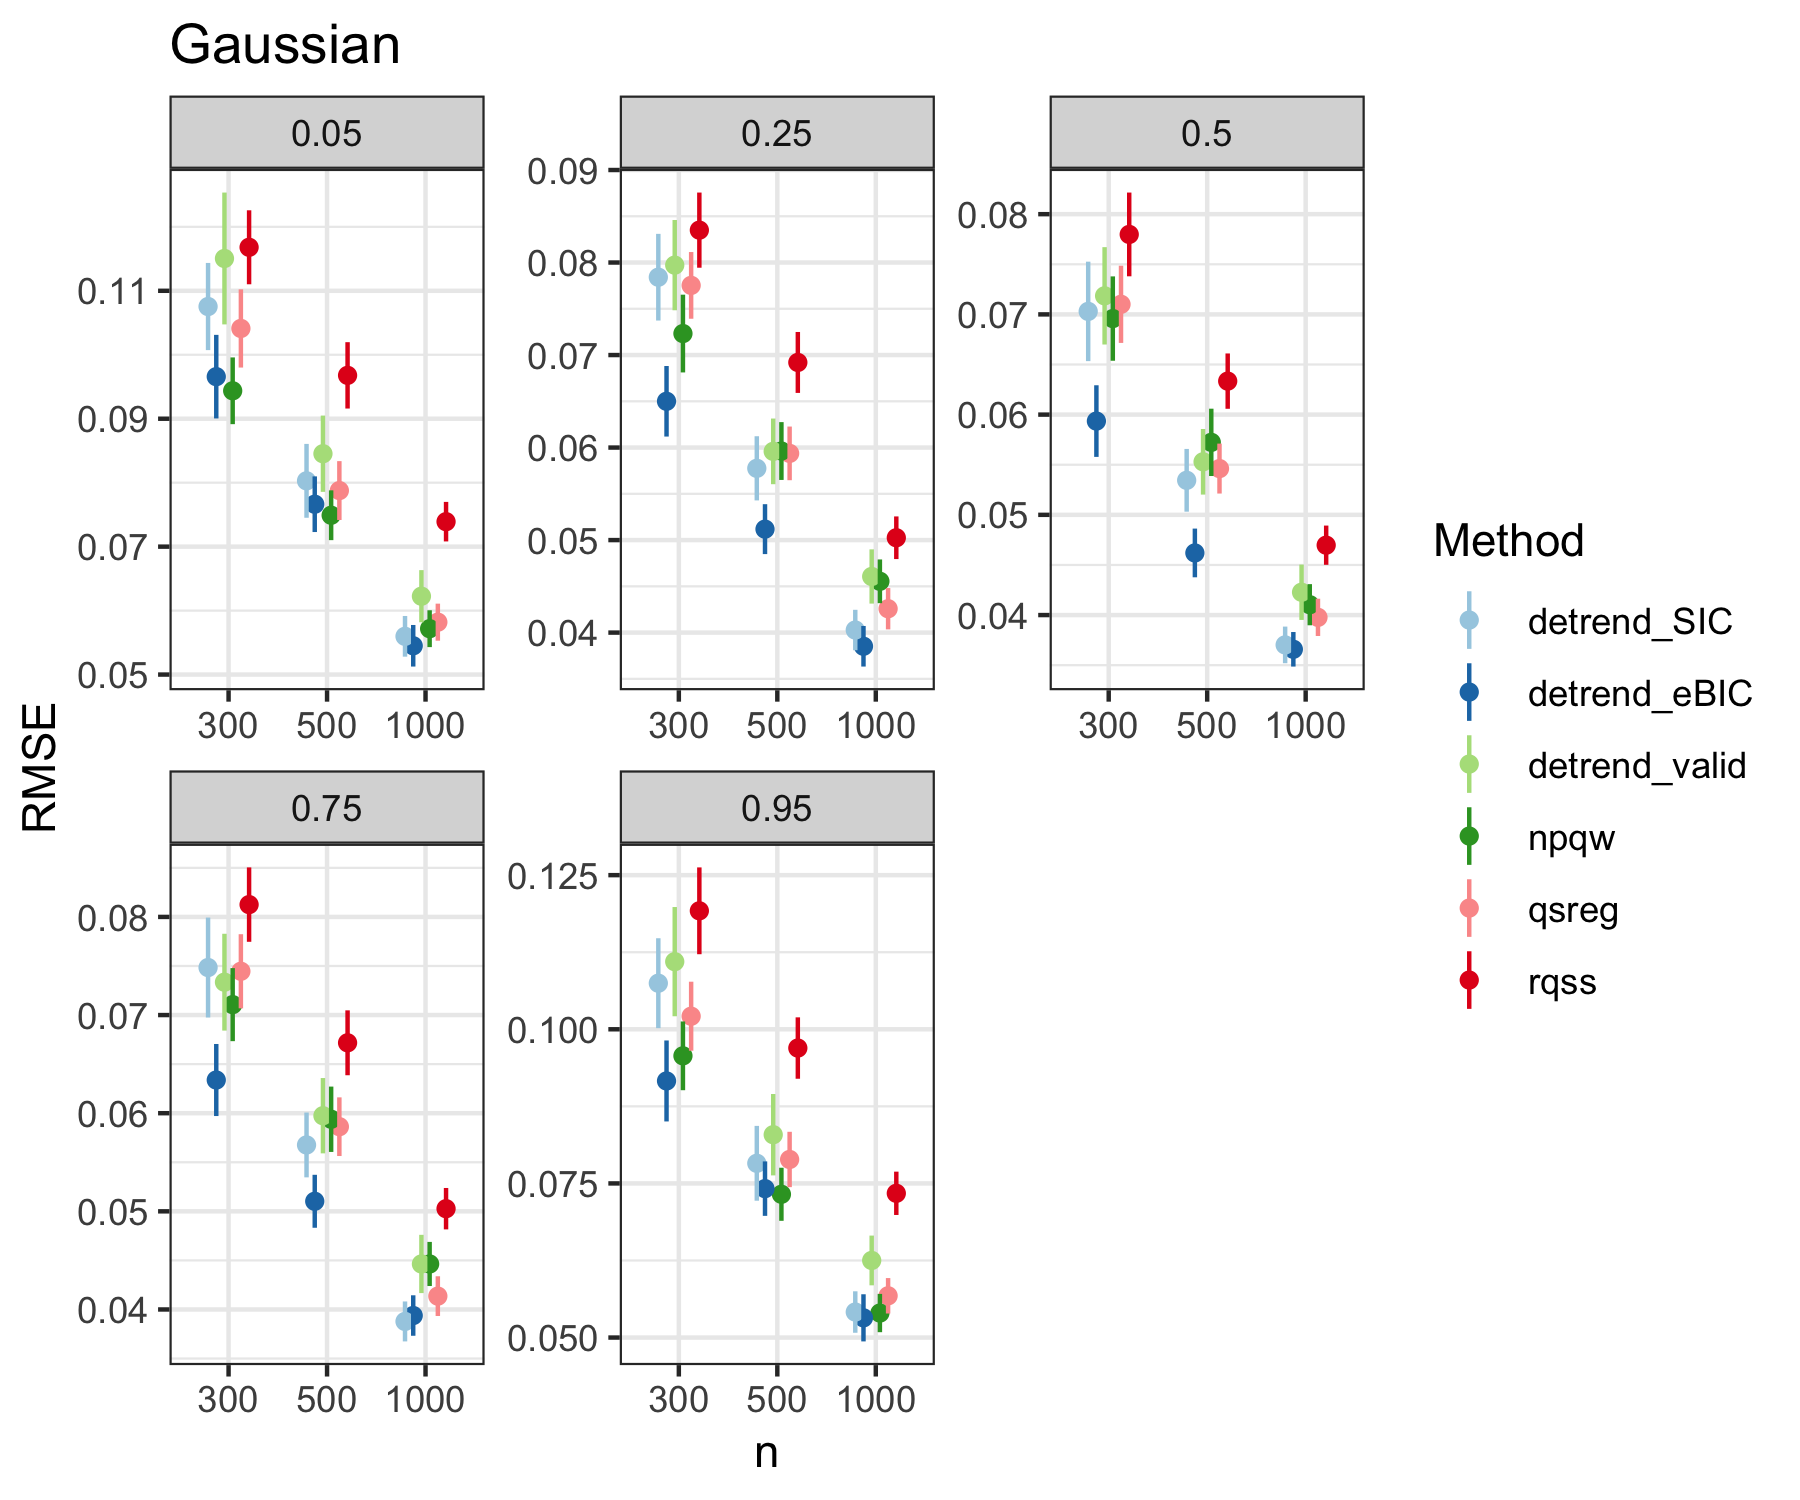
\includegraphics[width=\linewidth]{Figures/gaus_mse.png}	
		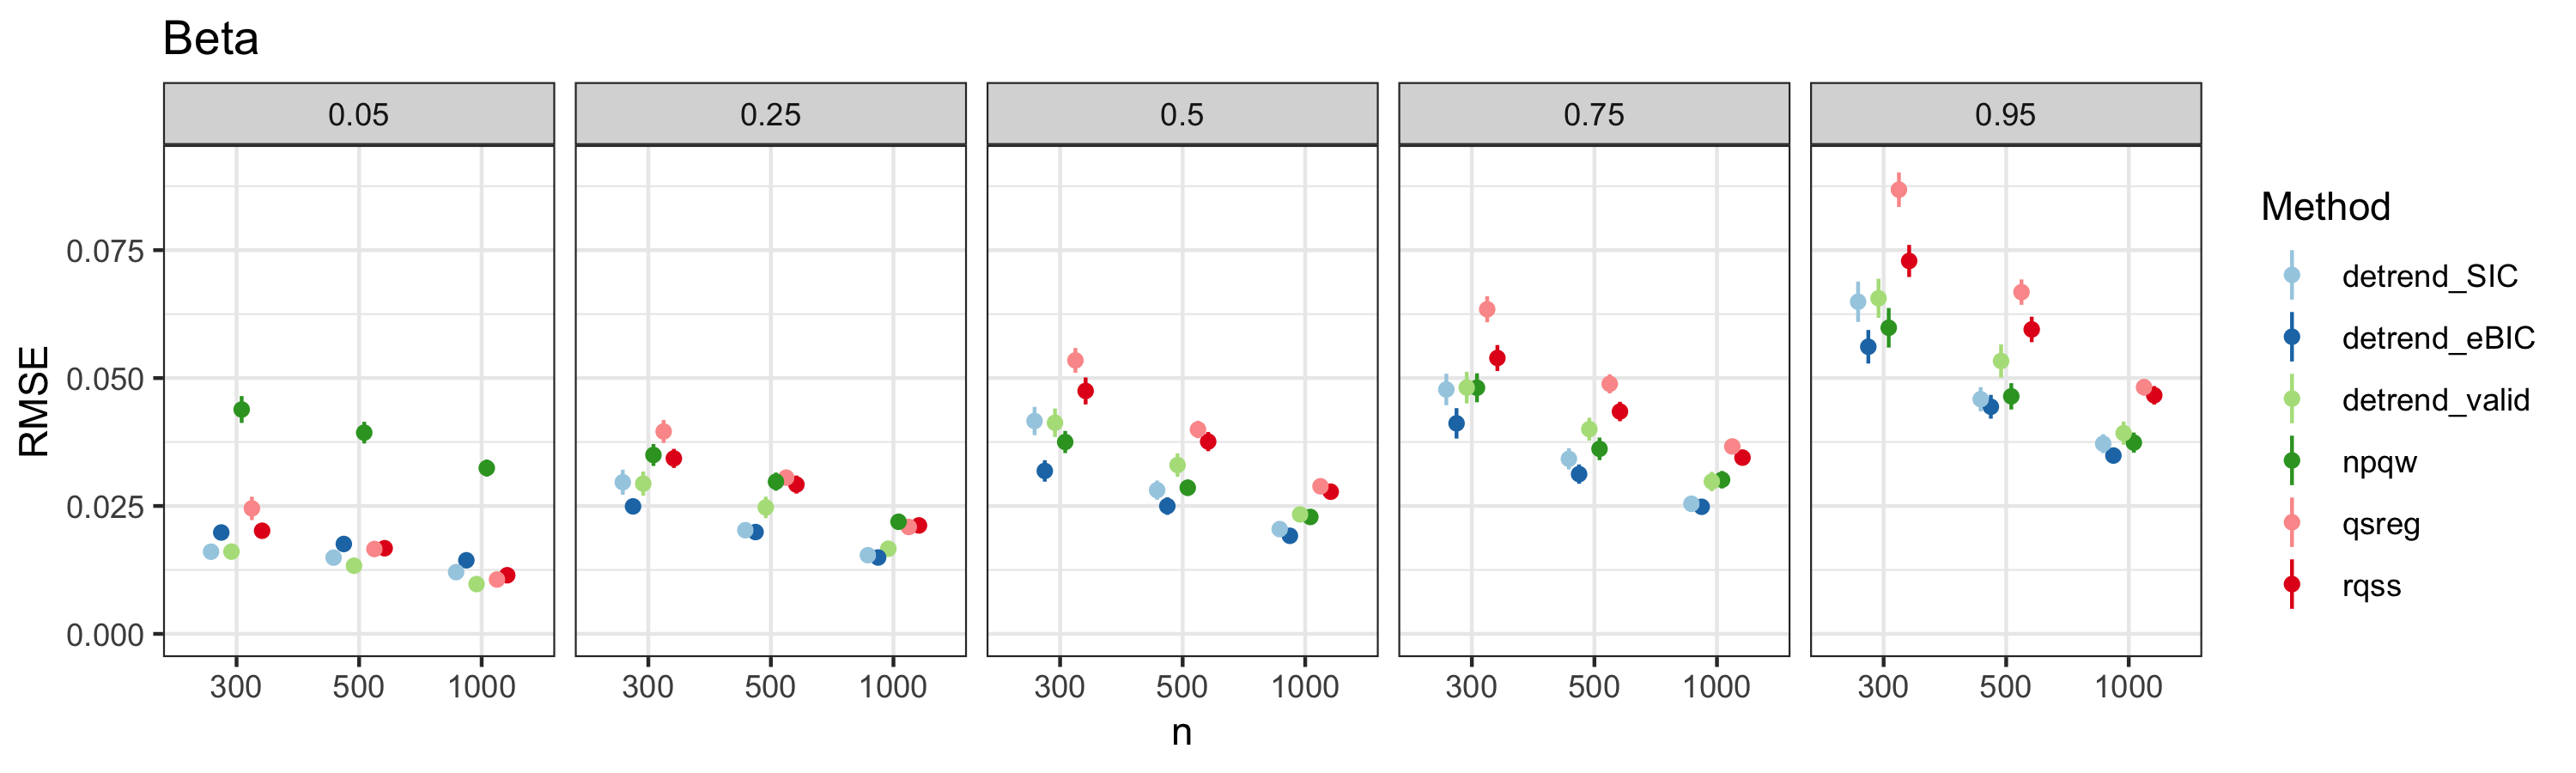
\includegraphics[width=\linewidth]{Figures/shapebeta_mse.png}
		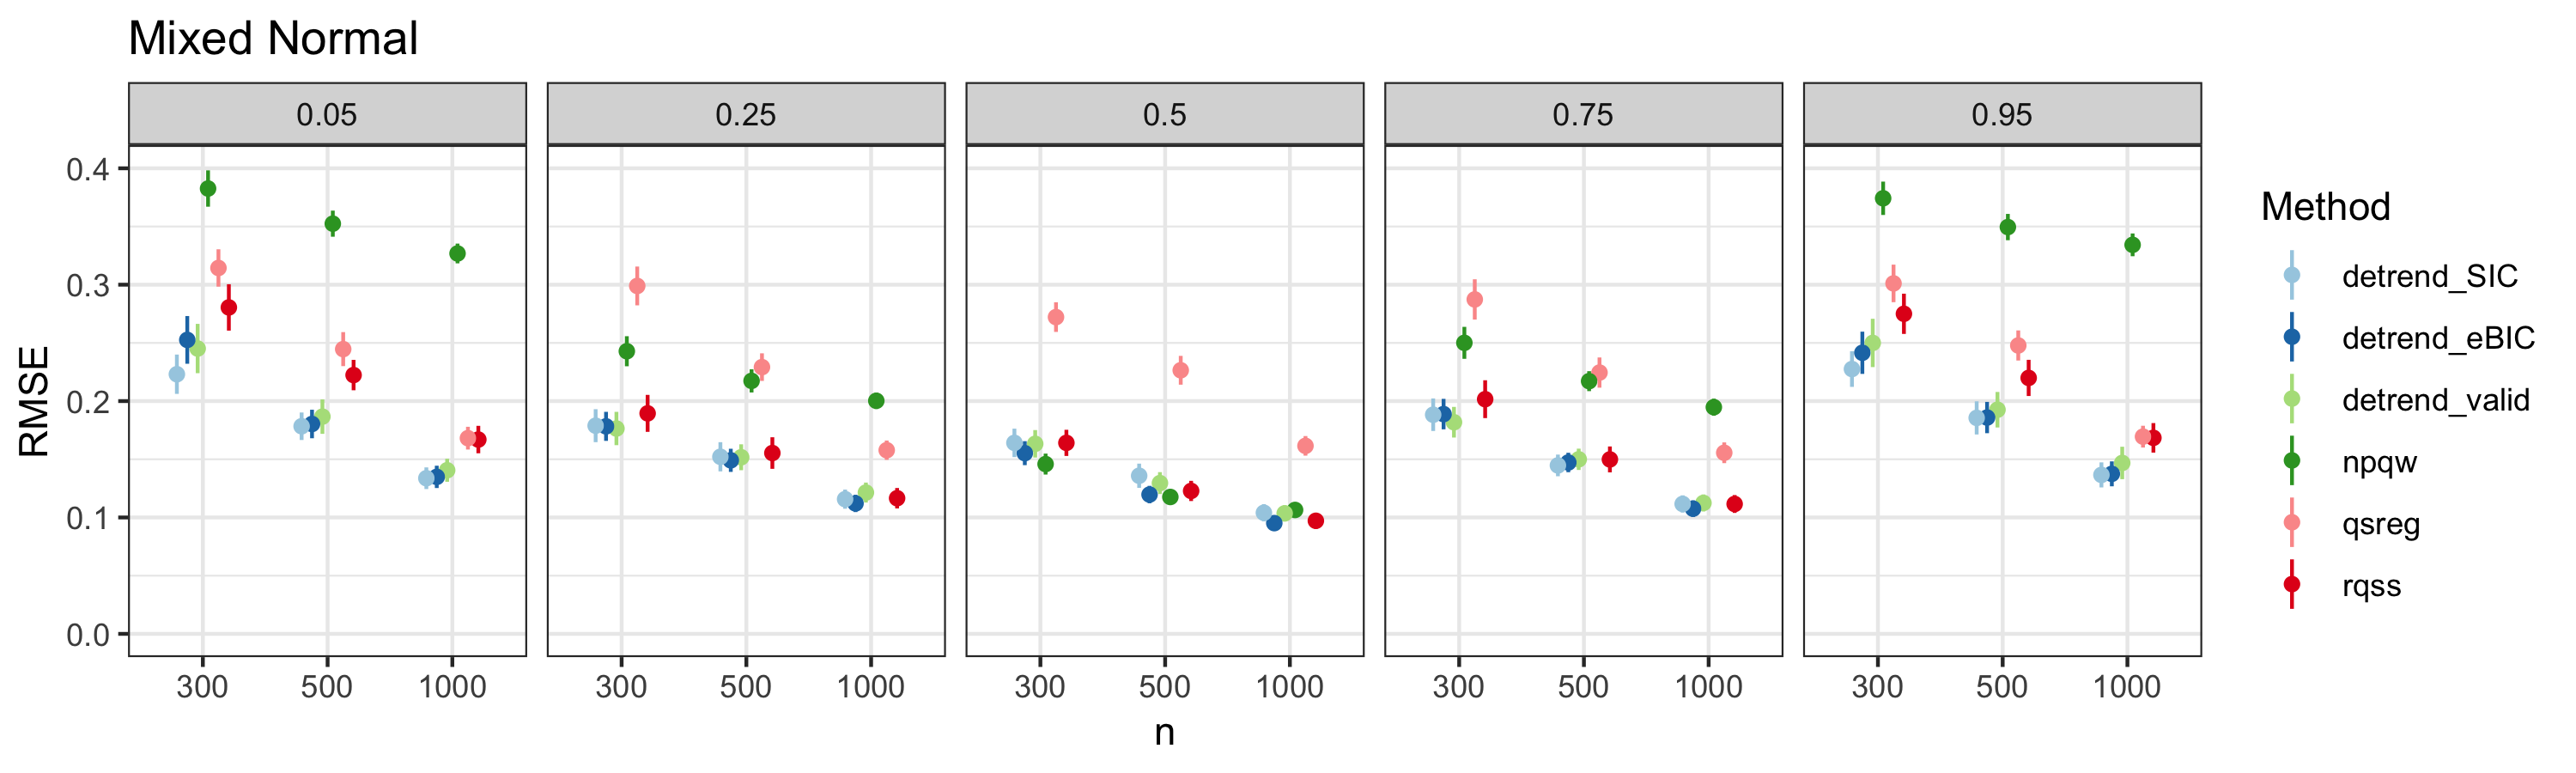
\includegraphics[width=\linewidth]{Figures/mixednorm_mse.png}
		\label{fig:quantile_mse}
	\end{figure}

	\subsection{Peak Detection}
%	\begin{figure}[h]
%		\caption{Example of simulated peaks, baseline, and observed measurements.}
%		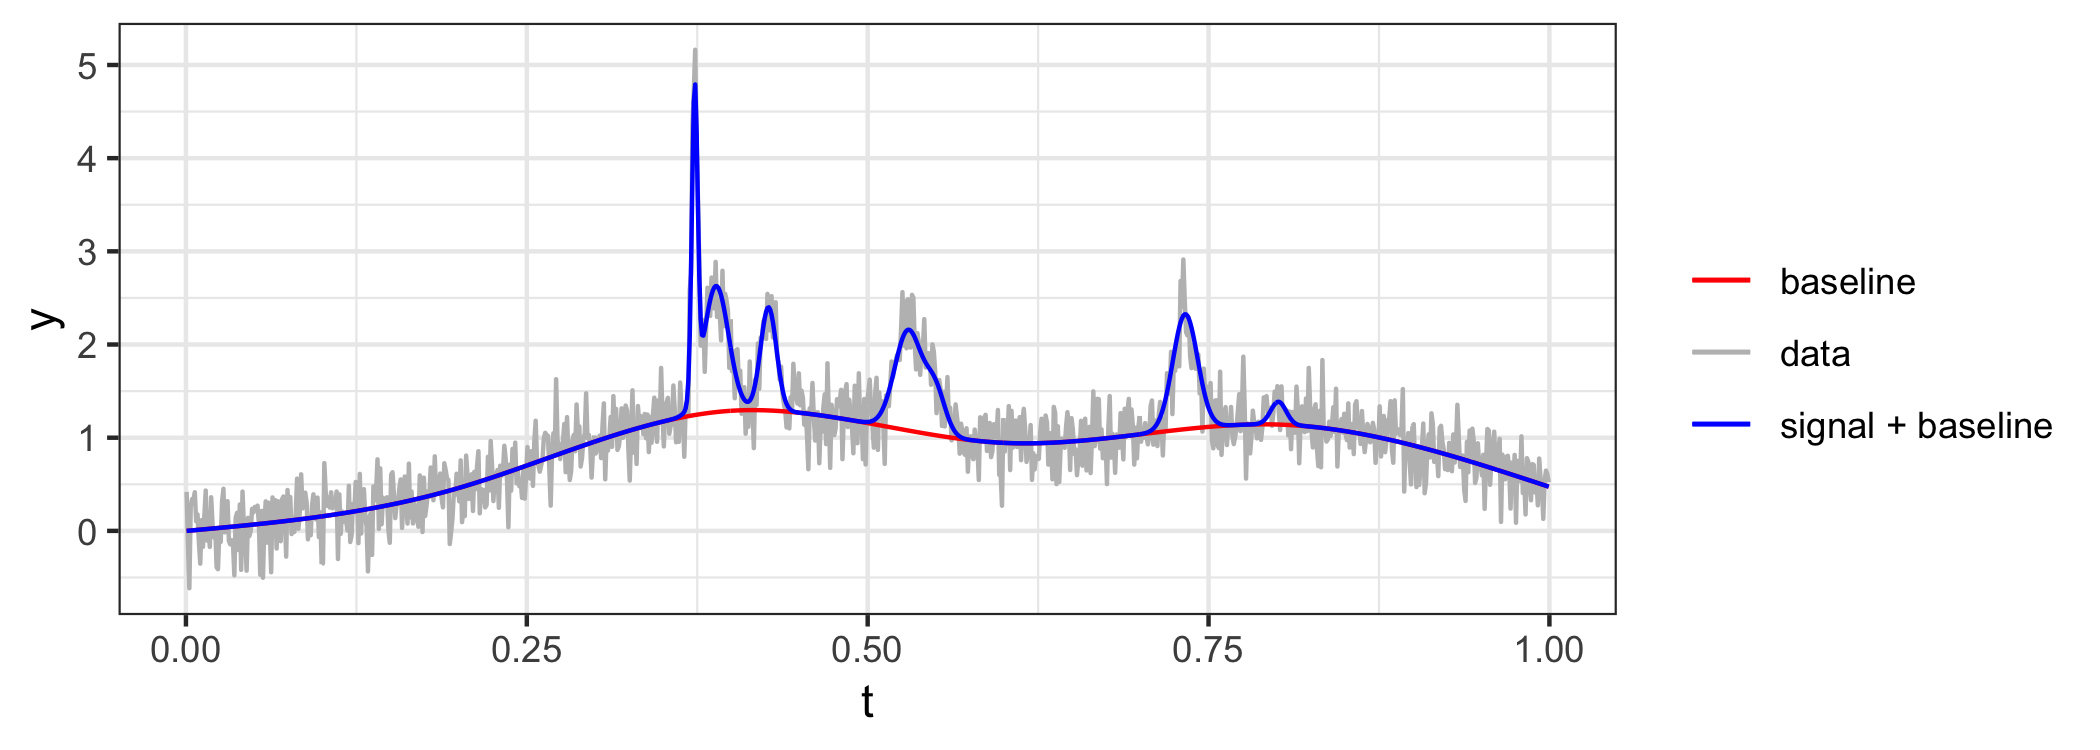
\includegraphics[width = \linewidth]{Figures/ex_peaks.png}
%	\end{figure}
	We use another simulation design based on the applied problem we aim to solve. We assume that the measured data can be represented by 
	\begin{equation}
	Y(t) = s(t) + b(t) + \epsilon(t)
	\end{equation} 
	with $t = 1, ..., n$, where $s(t)$ is the true signal at time $t$, $b(t)$ is the drift component that varies smoothly over time and $\epsilon(t) \sim N(0, 0.25^2)$ is an error component. We generate $b(t)$ using cubic natural spline basis functions with degrees of freedom sampled from a Poisson distribution with mean parameter equal to $n/100$,  and coefficients drawn from an exponential distribution with rate 1. The true signal function is assumed to be zero with peaks generated using the Gaussian density function. The number of peaks is sampled from a binomial distribution with size equal to $n$ and probability equal to $0.005$ with location parameters uniformly distributed between $1$ and $n-1$ and bandwidths uniformly distributed between $2$ and $12$. The simulated peaks were multiplied by a factor that was randomly drawn from a normal distribution with mean 20 and standard deviation of 4. One hundred datasets were generated for each $n=\{500, 1000, 2000, 4000\}$. We compare the ability of the methods to estimate the true quantiles of $Y(t)-s(t)$  for $\tau \in \{0.01, 0.05, 0.1\}$ and calculate the RMSE (Fig. \ref{fig:peaks_rmse}). In this simulation study our \texttt{detrend\_eBIC} method outperforms the others substantially. The \texttt{qsreg} method is comparable to the \texttt{detrend\_eBIC} method on the smaller datasets but its performance deteriorates as the data size grows. The \texttt{npqw} and \texttt{detrend\_valid} methods both perform poorly on this design. 
	
	\begin{figure}
		\caption{RMSE by method, quantile and data size for peaks design.}
		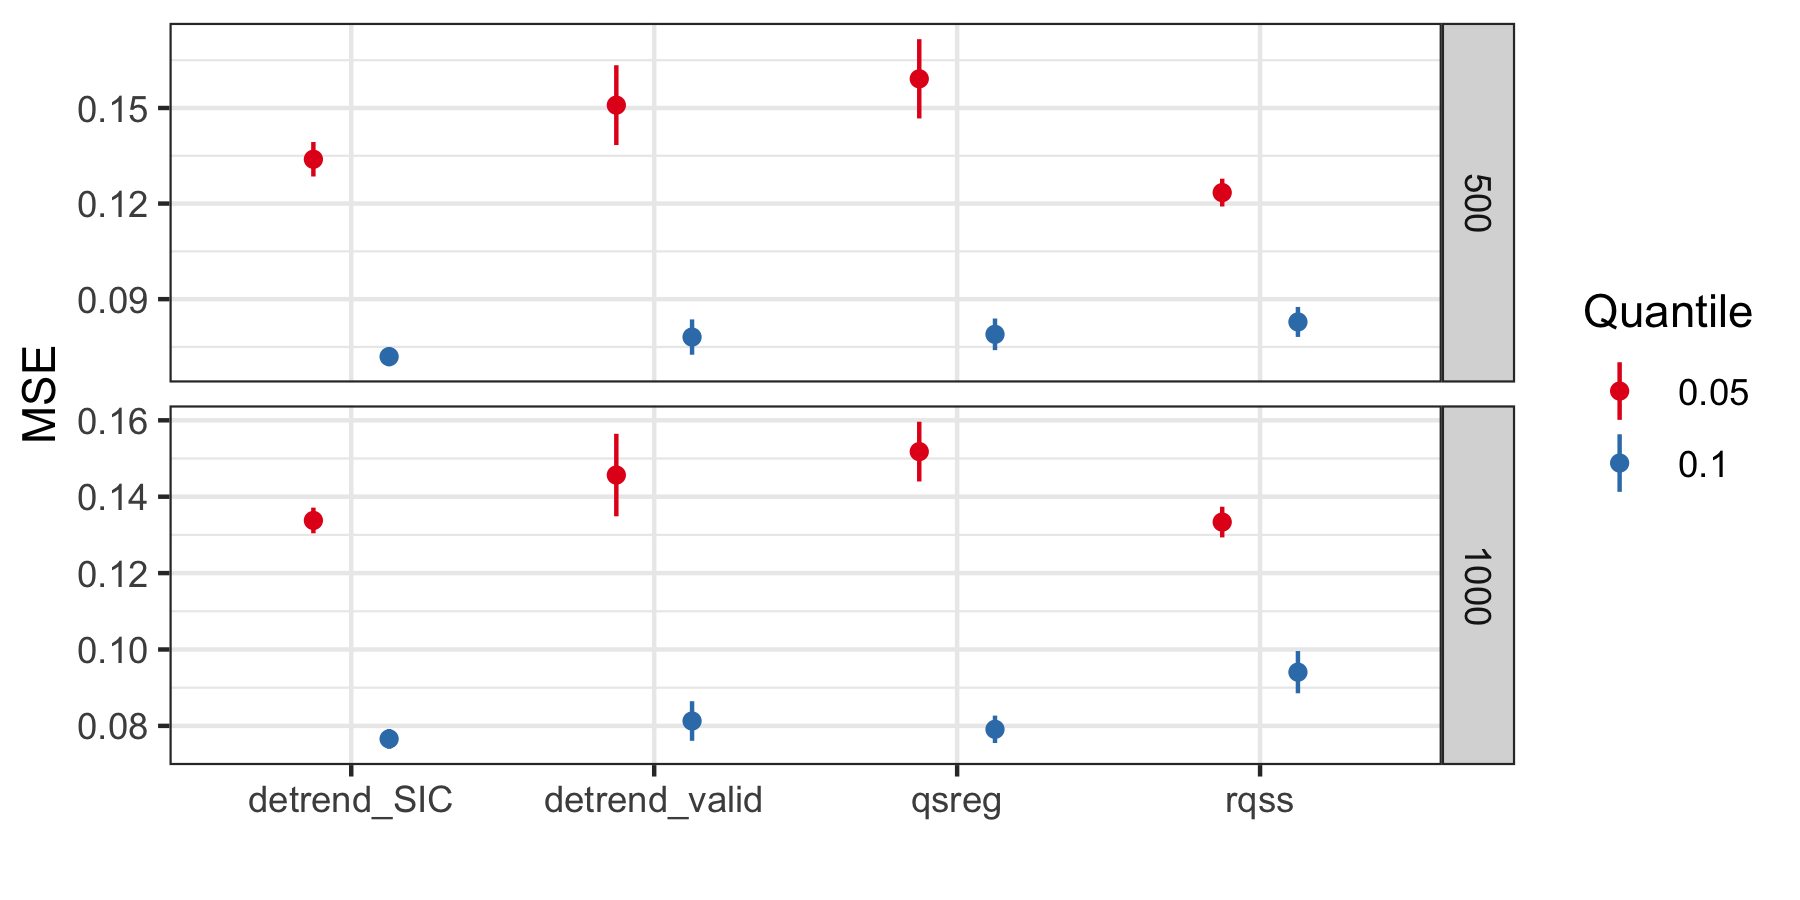
\includegraphics[width = \linewidth]{Figures/peaks_mse.png}	
		\label{fig:peaks_rmse}
	\end{figure}
	
	In our application, we want to accurately classify the observations into signal and no signal using a threshold. To evaluate the accuracy of our method compared to other methods we define true signal as any time point when the simulated peak value is greater than 0.5. We compare three different quantiles for the baseline estimation and four different thresholds for classifying the signal after subtracting the estimated baseline from the observations.  An illustration of the observations classified as signal after subtracting the baseline trend compared to the ``true signal" is shown in Fig. \ref{fig:peaks_class_eg}. To compare the resulting signal classifications we calculate the class averaged accuracy (CAA). Defining $s(t) \in \{0,1\}$ as the vector of true signal classification and $\hat{s}(t) \in \{0,1\}$ as the estimated signal classification, the CAA is defined as
	\begin{equation}
	\mbox{CAA} = \frac{1}{2}\left(\frac{\sum_{t=1}^n \mathbf{I}[s(t) = 1 \cap \hat{s}(t)=1]}{\sum_{t=1}^n \mathbf{I}[s(t) = 1]} + \frac{\sum_{t=1}^n \mathbf{I}[s(t) = 0 \cap \hat{s}(t)=0]}{\sum_{t=1}^n \mathbf{I}[s(t) = 0]}\right).
	\end{equation}  
	We use this metric because our classes tend to be very un-balanced with many more $0$s than $1$s. The CAA metric will always give a score of 0.5 for random guessing and also for trivial classifiers such as $\hat{s}(t) = 0$ for all $t$. 

	Our \texttt{detrend\_BIC} method performs the best overall in terms of both RMSE and CAA. While \texttt{qsreg} was competitive with our method in some cases, in the majority of cases the largest CAA values for each threshold were produced using the \texttt{detrend\_eBIC} method with the 1\textsuperscript{st} or 5\textsuperscript{th} quantiles. 
	
	\begin{figure}[h!]
		\caption{Example signal classification using threshold. Red indicates true signal $>0.5$, blue indicates observations classified as signal after baseline removal using \texttt{detrend\_eBIC} and a threshold of 1.2.}
		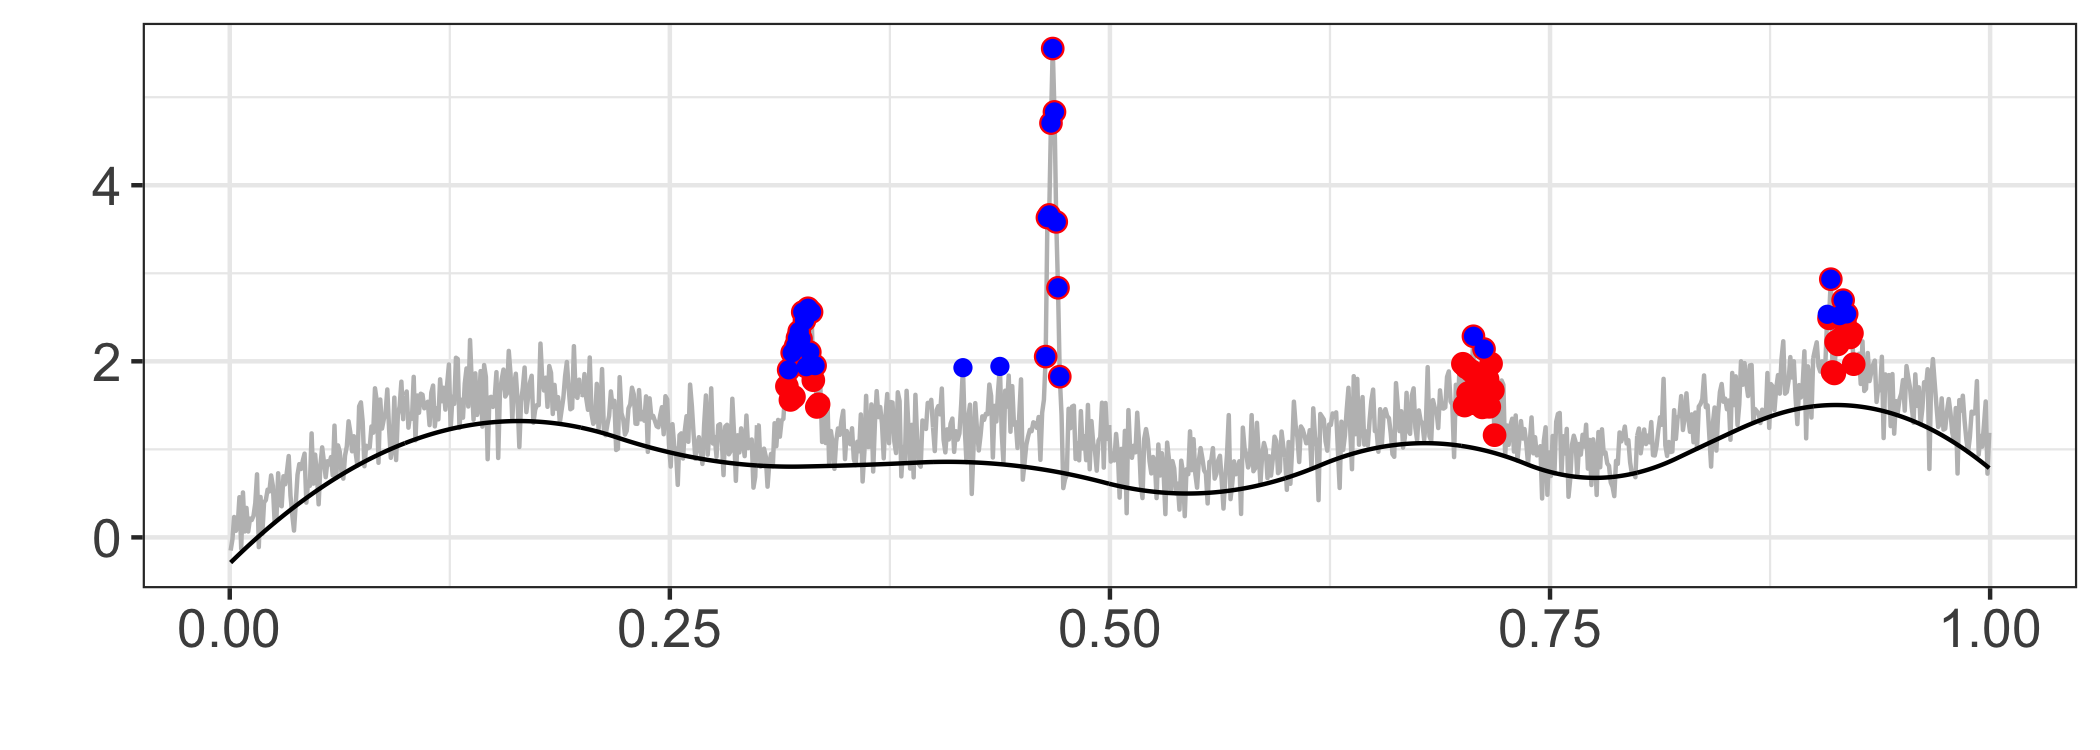
\includegraphics[width = \linewidth]{Figures/peaks_eg_class.png}
		\label{fig:peaks_class_eg}
	\end{figure}
	

	\begin{figure}[h!]
		\caption{Class averaged accuracy by threshold, data size, and method (1 is best 0.5 is worst).}
		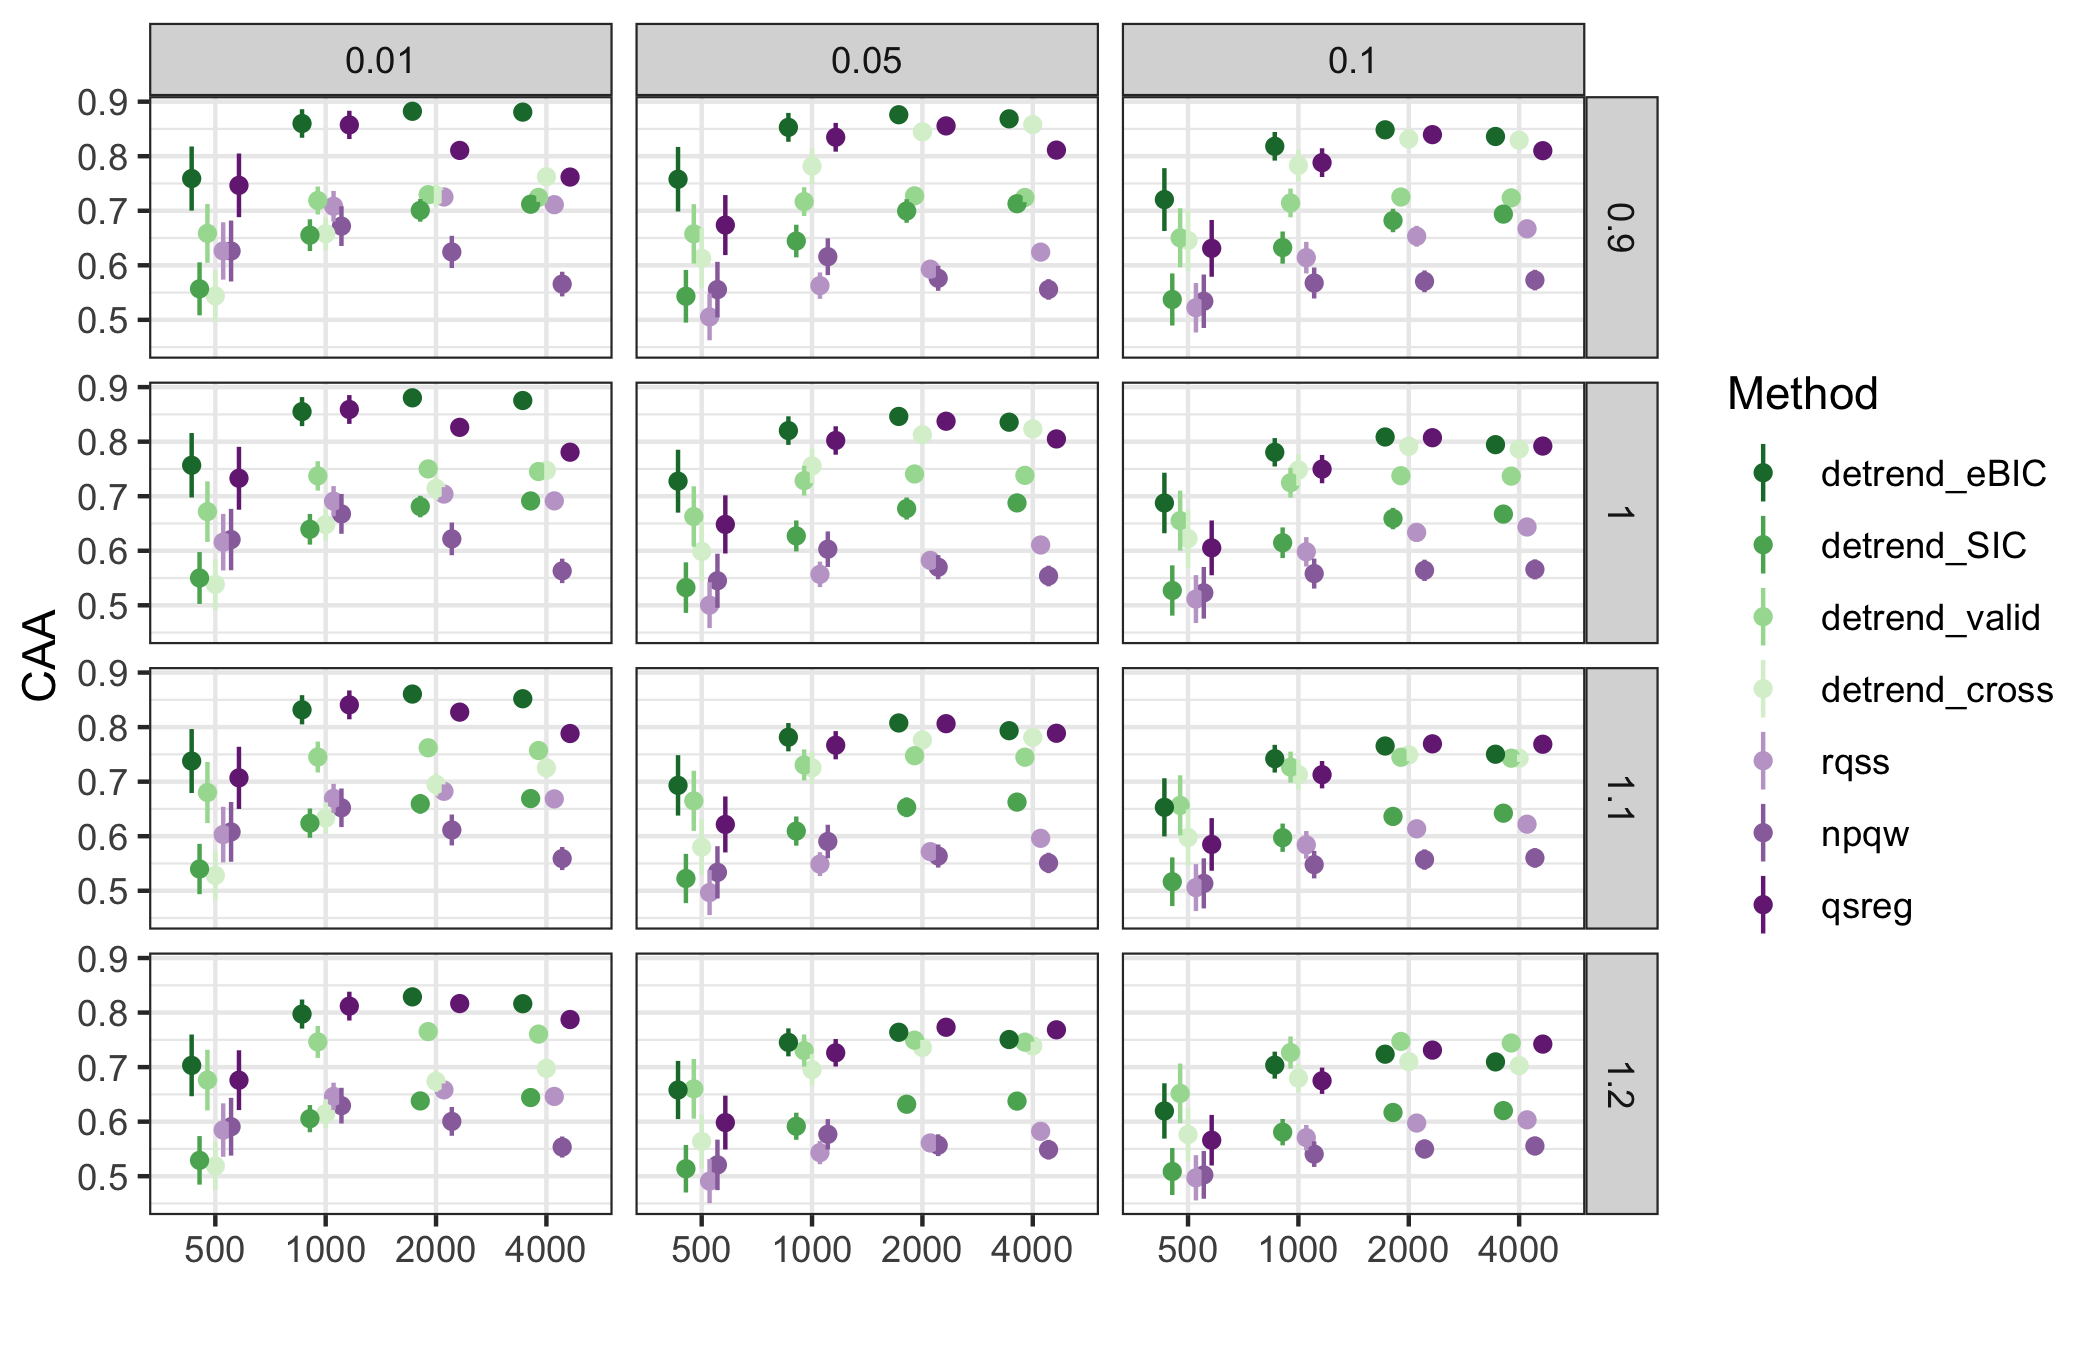
\includegraphics[width = \linewidth]{Figures/peaks_CAA.png}
	\end{figure}


	\FloatBarrier
	
	\section{Application}
	
	The low-cost ``SPod" air quality sensors output a time series that includes a slowly varying baseline, high frequency random noise, and the sensor response to pollutants. A potential use for these sensors is to monitor pollutant concentrations at the fence lines of industrial facilities and detect time points when high concentrations are present. Ideally, three co-located and time aligned sensors (as shown in Fig. \ref{fig:raw_spod}) responding to a pollutant plume would result in the same signal classification after baseline trend removal and proper threshold choice. 
	
	\begin{figure}
		\caption{Estimated 15\textsuperscript{th} quantile trends on subset of the data using \texttt{qsreg} and \texttt{detrend\_eBIC}.} 
		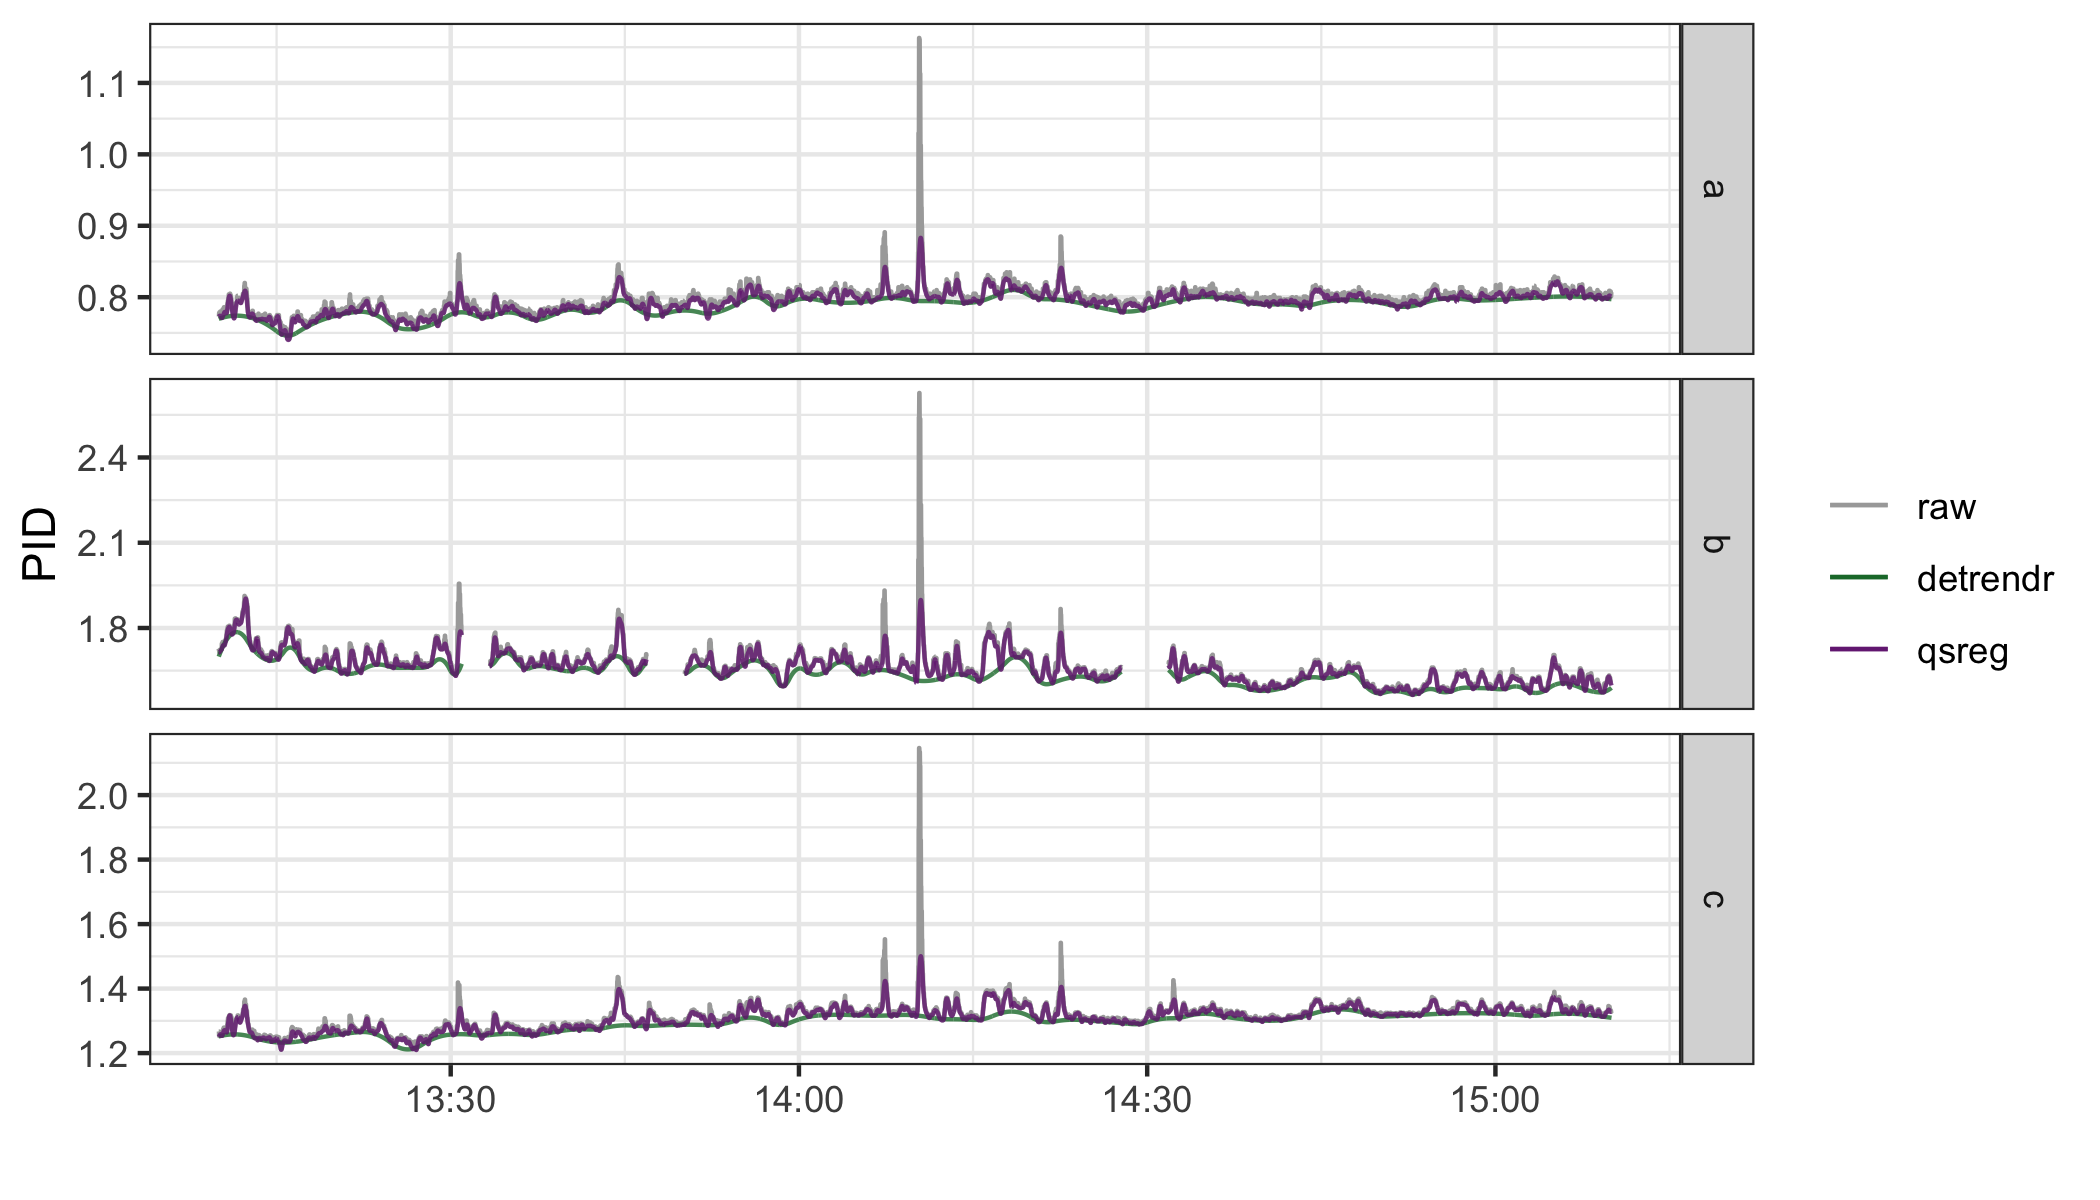
\includegraphics[width = \linewidth]{Figures/short_trends.png}
		\label{fig:short-trends}
	\end{figure}

	We compare our \texttt{detrend\_eBIC} method with the \texttt{qsreg} method on a subset of the SPod data (n=6000) since the \texttt{qsreg} method cannot handle all 24 hours simultaneously. We estimate the baseline trend using the 10\textsuperscript{th} and 15\textsuperscript{th} quantiles and compare three thresholds for classifying signal. The thresholds are calculated using the median plus a multiple of the median absolute deviation (Eq. \ref{eq:MAD}) of the detrended series. 
	\begin{equation}
	\label{eq:MAD}
	\mbox{MAD} = \mbox{median}(y-\tilde{y}),
	\end{equation}
	where $\tilde{y}$ is the median of $y$. Given a method, quantile level, and MAD multiple, we estimate the quantile trend for each of the sensor nodes and subtract it from the observations. We then calculate the threshold using the median plus the MAD multiple of the corrected series and classify the corrected series based on the threshold. An example of the estimated baseline fit for each method is shown in Fig. \ref{fig:short-trends}, while Fig. \ref{fig:rugplot} shows the series after subtracting the \texttt{detrend\_eBIC} estimate of the 15\textsuperscript{th} quantile and classifying the signal using a MAD multiple of 3. 
	 
 	\begin{figure}
	 	\caption{Rugplot showing locations of signal after baseline removal using detrendr estimate of 15th quantile. Horizontal dashed lines represent the thresholds.}
	 	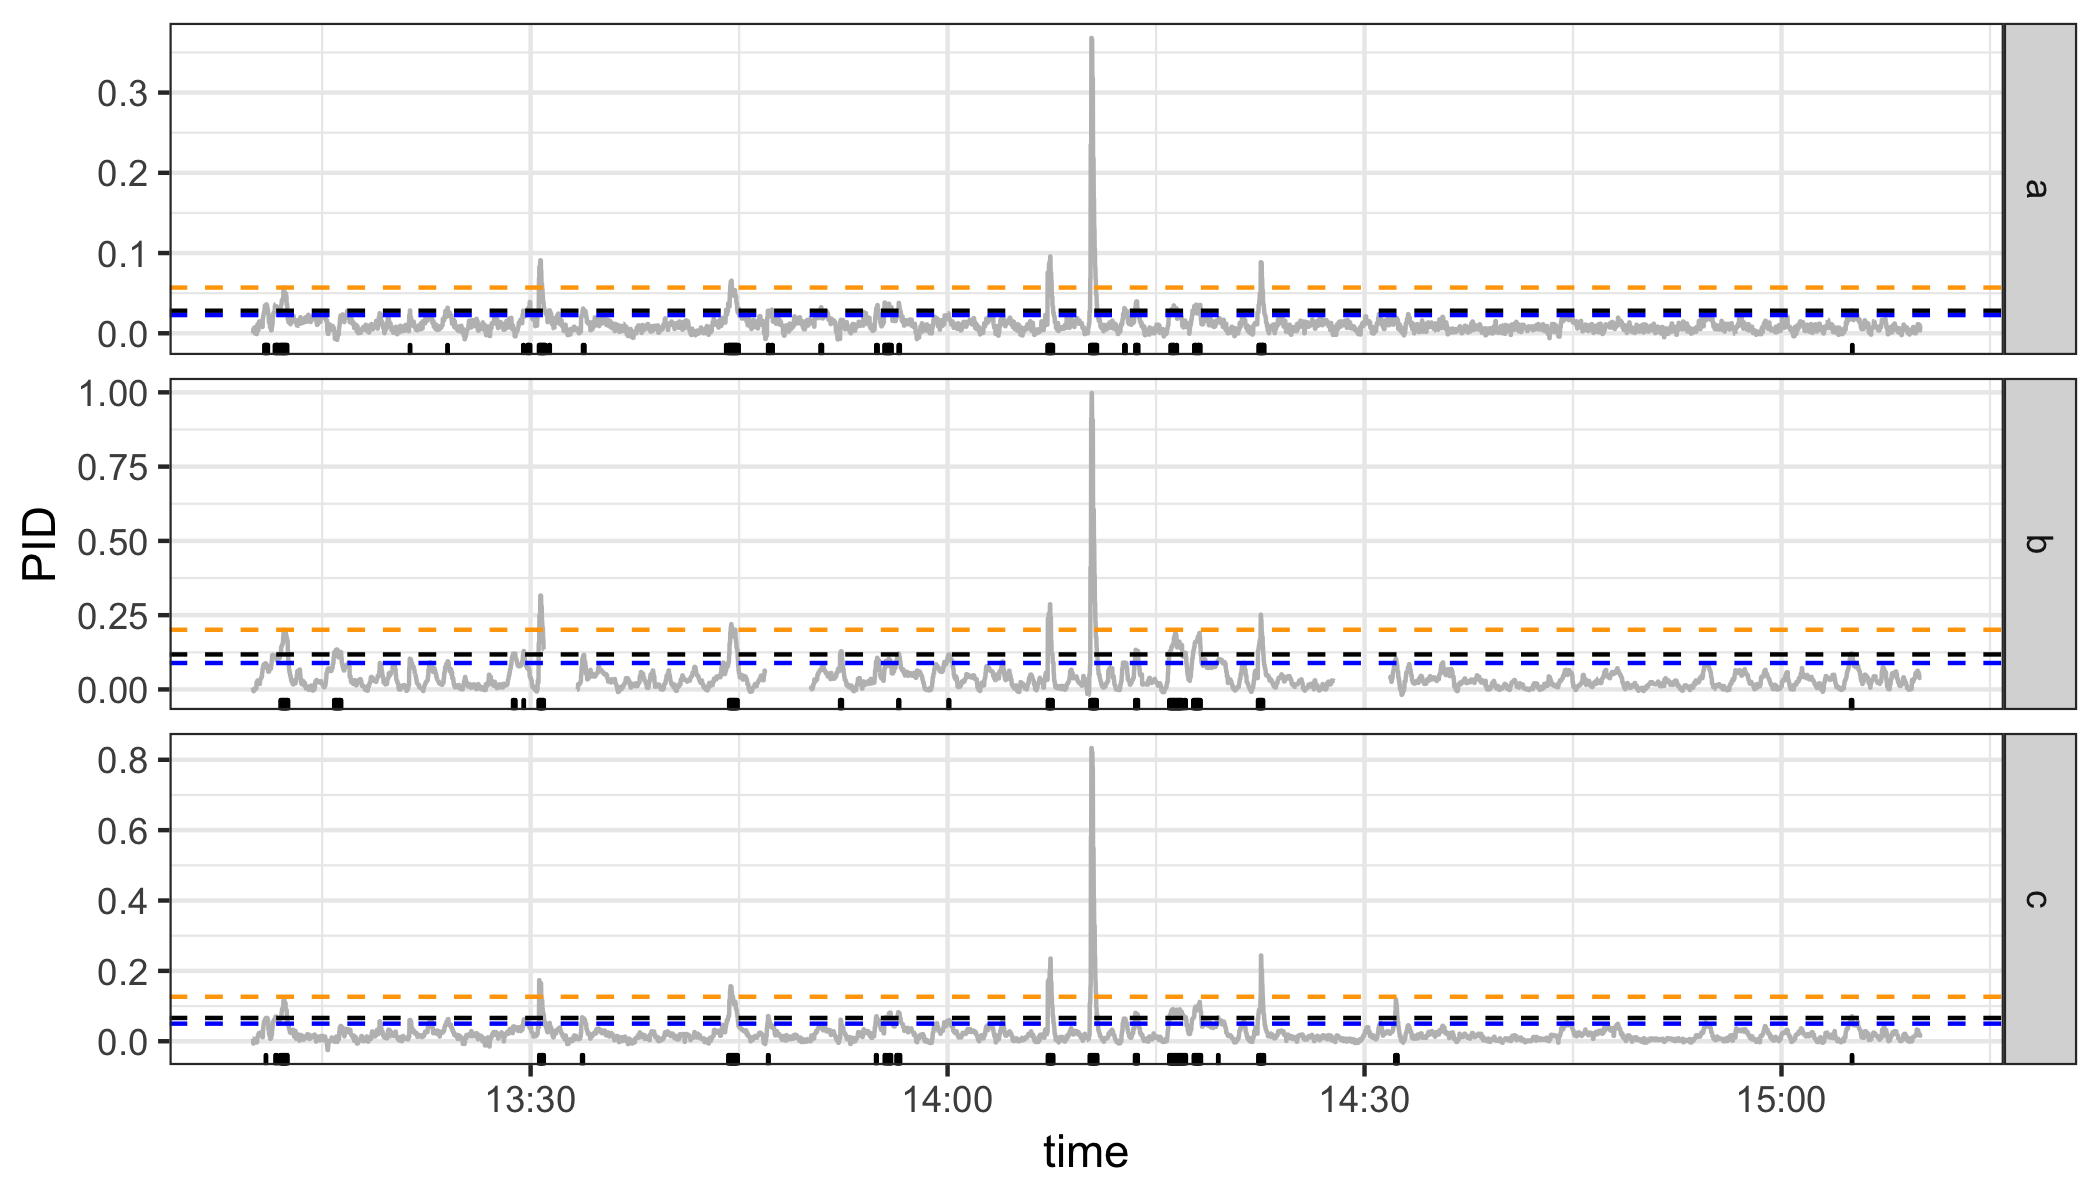
\includegraphics[width = \linewidth]{Figures/corrected_rugplot.png}
	 	\label{fig:rugplot}
	 \end{figure}
	 
	Given the signal classifications for node 1, $s_1(t) \in \{0,1\}$ and node 2, $s_2(t)\in\{0,1\}$ we want to compare the similarity between the two classifications. One metric for evaluating the distance between two classifications is the variation of information (VI): 
	\begin{align*}
		r_{ij} =& \frac{1}{n}\sum_t \mathbf{I}(s_1(t) = i  \cap s_2(t) = j)\\
		VI(s_1, s_2) =& -\sum_{i,j} r_{ij} \left[ \log \left(\frac{r_{ij}}{\frac{1}{n}\sum_t \mathbf{I}(s_1(t) = i)}\right) + 
		\log \left(\frac{r_{ij}}{\frac{1}{n}\sum_t \mathbf{I}(s_2(t) = j)}\right) \right]
	\end{align*}	
	The VI is a distance metric for measuring similarity of classifications and will be 0 if the classifications are identical and increase as the classifications become more different. The VIs by method, quantile and trend are shown in Fig. \ref{fig:vi}. In all cases our \texttt{detrend} method results in classifications that are more similar than those from the \texttt{qsreg} method. As is illustrated in Fig. \ref{fig:short-trends} and Fig. \ref{fig:rugplot}, our method results in a smoother baseline estimate which improves signal classification. 
		
	\begin{figure}
		\centering
		\caption{Variation of Information between sensor nodes after trend removal by quantile and method and thresholding by factor of MAD.}
		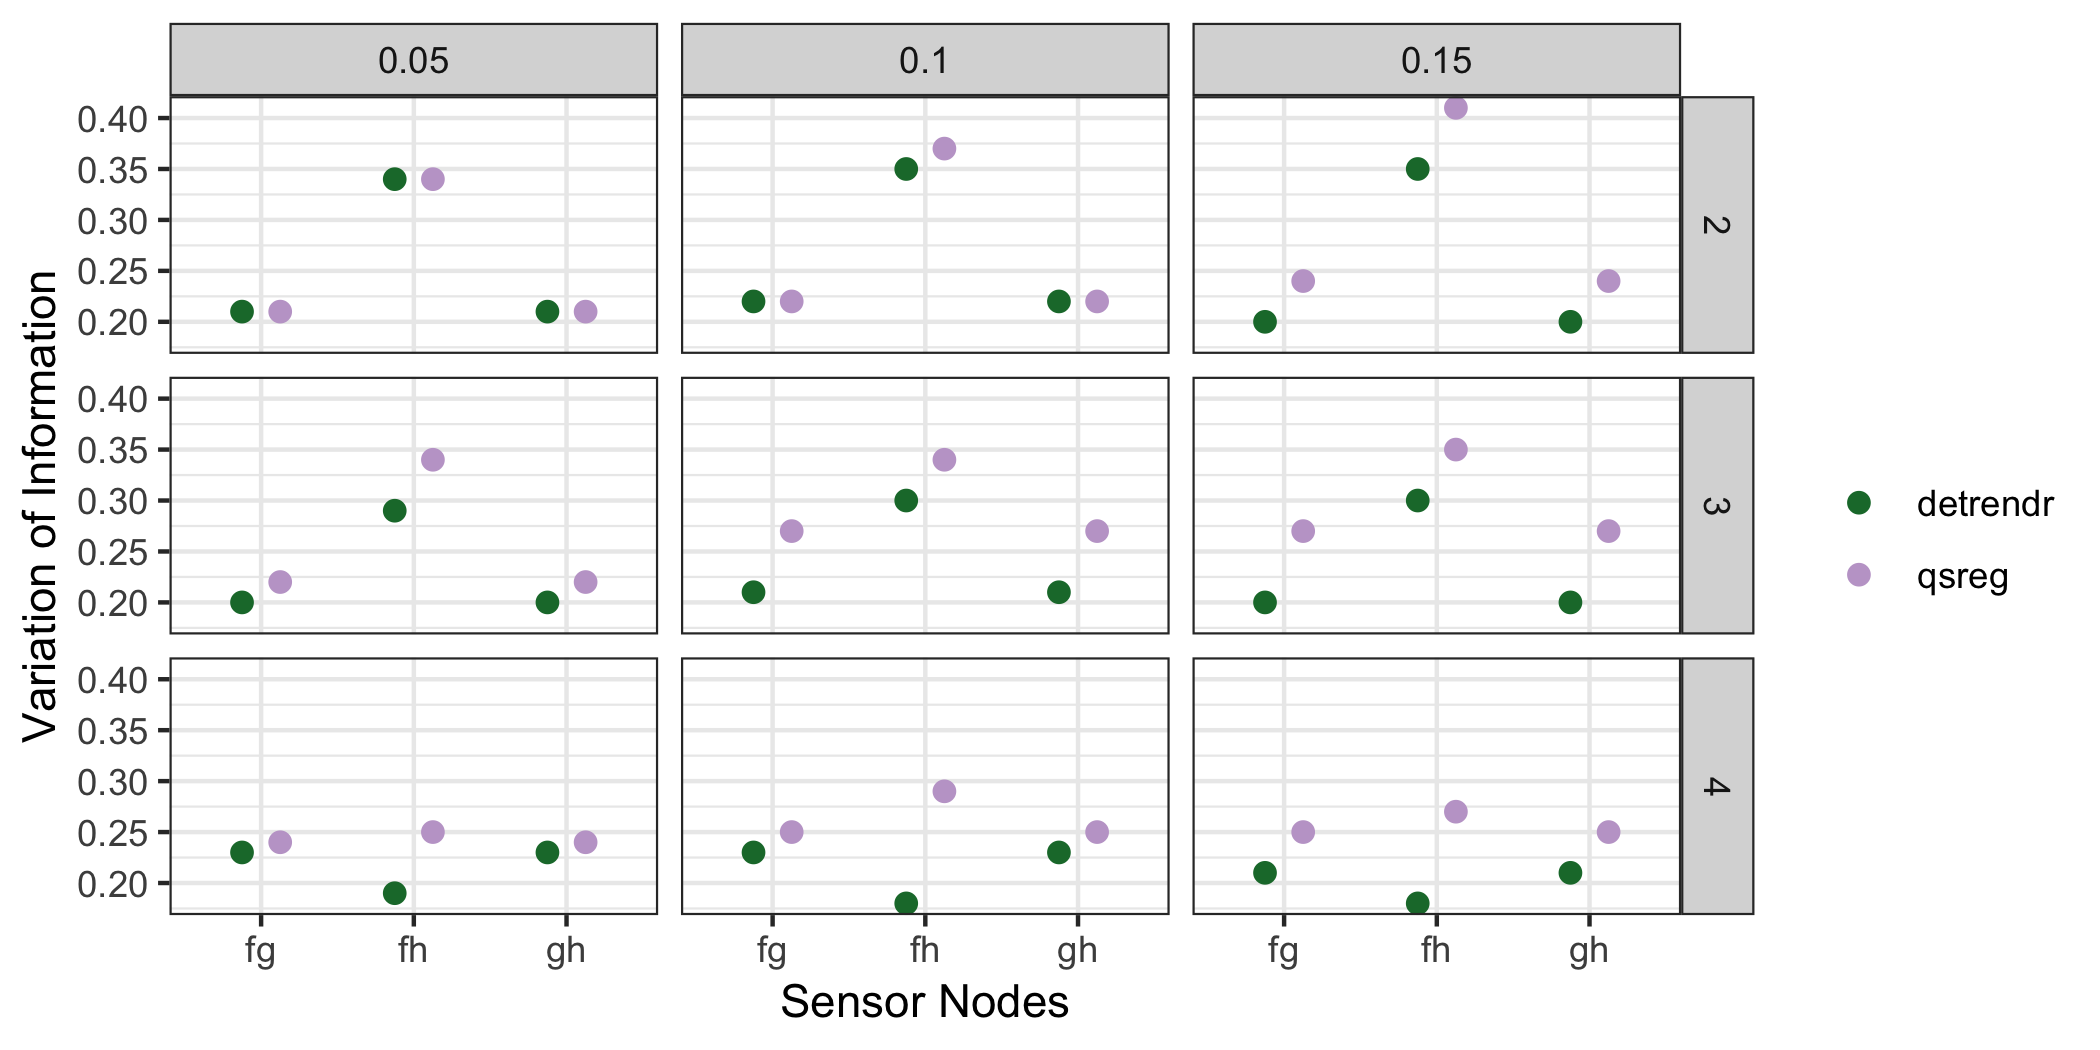
\includegraphics[width = .9\linewidth]{Figures/VI_app_short.png}
		\label{fig:vi}
	\end{figure}
	
	Our windowed \texttt{detrend\_eBIC} method was used to removed the baseline drift from the total dataset consisting of 86,401 observations per node. The VI scores for the full dataset were 0.36, 0.24, and 0.41 for nodes c and d, c and e, and d and e, respectively. The complete confusion matrices for the nodes using a MAD multiple of 5 for the threshold is given in Table 1. 
		
	\begin{figure}
		\caption{Low cost sensor data after drift removal using windowed detrend with eBIC.}
		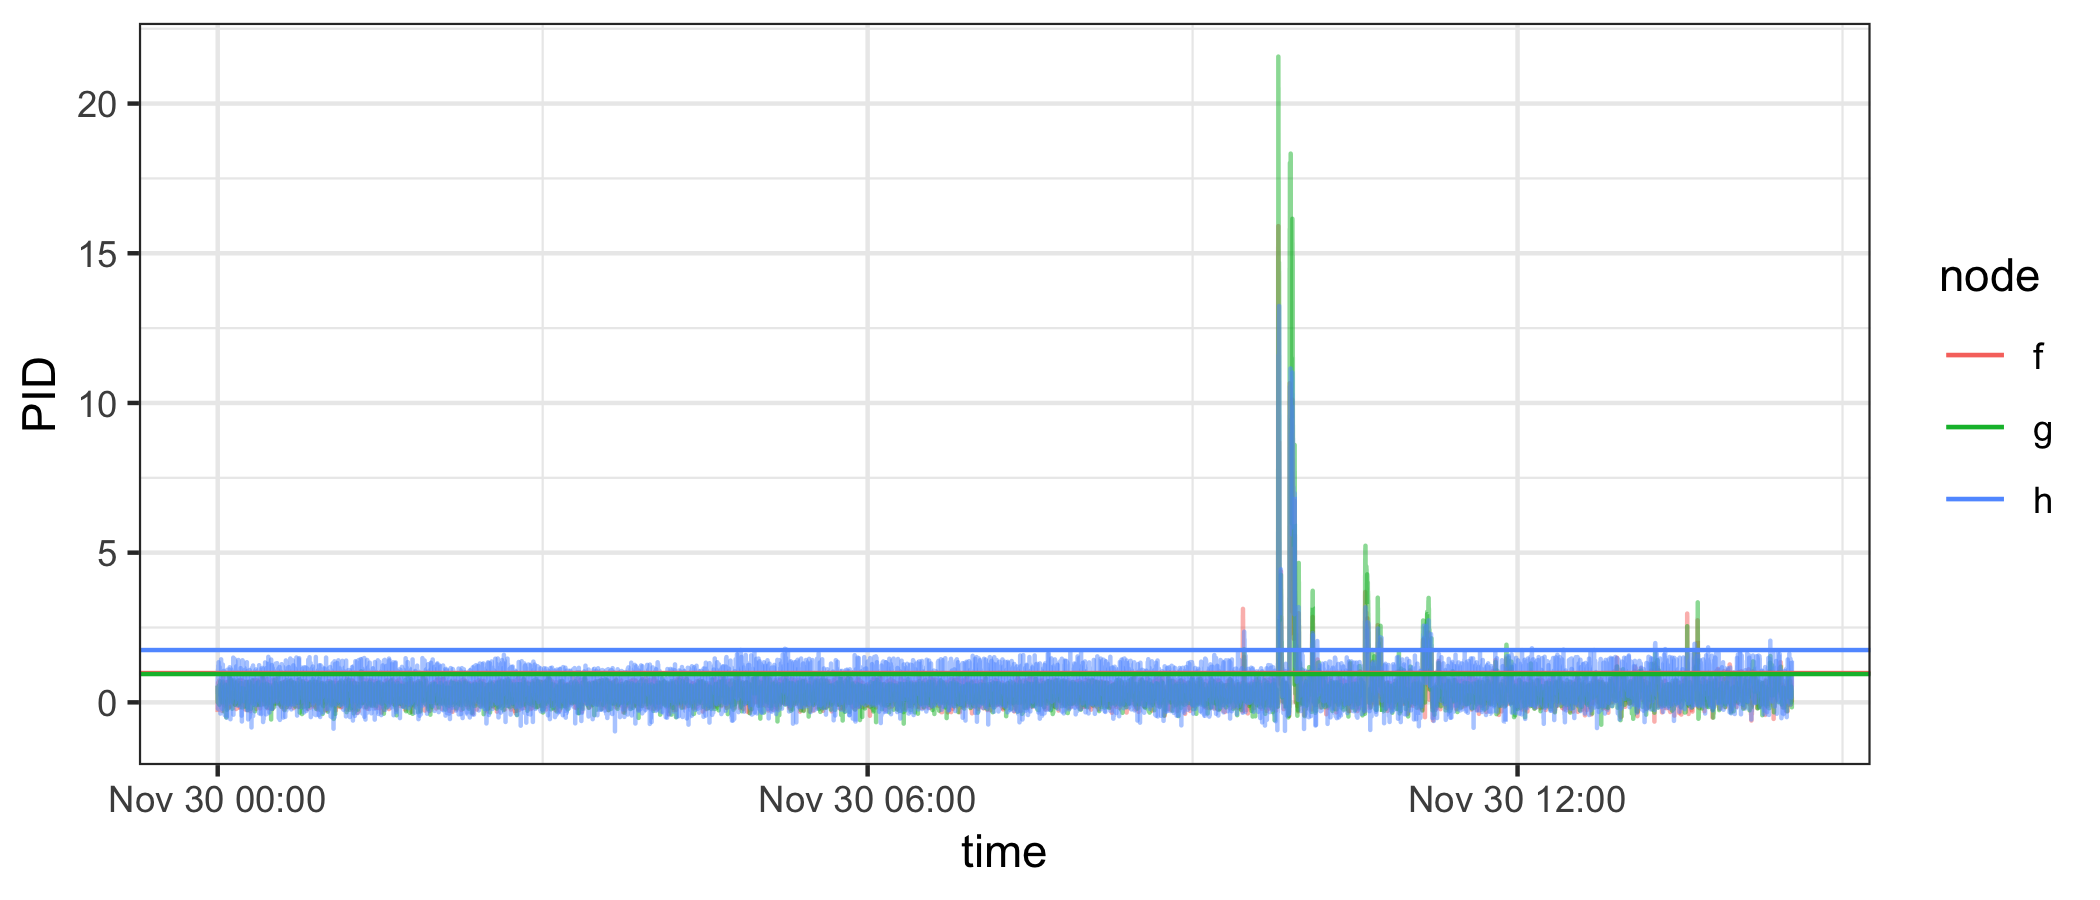
\includegraphics[width = \linewidth]{Figures/corrected_data.png}
	\end{figure}

	%latex.default(conf, file = "../Manuscript/full_confusion_detrend.tex",     rowlabel = "", rowname = c("f = 0", "f = 1", "f=0", "f=1"),     cgroup = c("h = 0", "h = 1"), rgroup = c("tau=0.05", "tau=0.1"),     n.rgroup = c(2, 2), colheads = rep(c("g = 0", "g = 1"), 2),     n.cgroup = c(2, 2), caption = "Confusion matrices for 3 SPod nodes after baseline removal (n=52322).")%
\begin{table}[!tbp]
\caption{Confusion matrices for 3 SPod nodes after baseline removal (n=52322).\label{conf}} 
\begin{center}
\begin{tabular}{lrrcrr}
\hline\hline
\multicolumn{1}{l}{\bfseries }&\multicolumn{2}{c}{\bfseries h = 0}&\multicolumn{1}{c}{\bfseries }&\multicolumn{2}{c}{\bfseries h = 1}\tabularnewline
\cline{2-3} \cline{5-6}
\multicolumn{1}{l}{}&\multicolumn{1}{c}{g = 0}&\multicolumn{1}{c}{g = 1}&\multicolumn{1}{c}{}&\multicolumn{1}{c}{g = 0}&\multicolumn{1}{c}{g = 1}\tabularnewline
\hline
{\bfseries tau=0.05}&&&&&\tabularnewline
~~f = 0&$51641$&$222$&&$1$&$  9$\tabularnewline
~~f = 1&$   23$&$190$&&$7$&$229$\tabularnewline
\hline
{\bfseries tau=0.1}&&&&&\tabularnewline
~~f=0&$51639$&$231$&&$1$&$  9$\tabularnewline
~~f=1&$   23$&$187$&&$7$&$225$\tabularnewline
\hline
\end{tabular}\end{center}
\end{table}
	
	

	\section{Conclusion and Discussion}
	We have expanded the quantile trend filtering method by implementing a non-crossing constraint and a new algorithm for processing large series, and proposing a modified criteria for smoothing parameter selection. Furthermore we have demonstrated the utility of quantile trend filtering in both simulations and applied settings. Our ADMM algorithm for large series both reduces the computing time and allows trends to be estimated on series that cannot be estimated simultaneously while our scaled extended BIC criteria was shown to provided better estimated of quantile trends in series with and without a signal component. We have also shown that the baseline drift in low cost air quality sensors can be removed through estimating quantile trends.
	 
	In the future, quantile trend filtering could be extended to observations measured at non-uniform spacing by incorporating the distance in covariate spacing into the differencing matrix. It could also be extended to estimate smooth spatial trends by a similar adjustment to the differencing matrix based on spatial distances between observations. 
	
	\label{sec:conc}
	
	
	\bigskip
	\begin{center}
		{\large\bf SUPPLEMENTARY MATERIAL}
	\end{center}
	
	\begin{description}
		
		\item[R-package for detrend routine:] R-package detrendr containing code to perform the diagnostic methods described in the article. (GNU zipped tar file)
				
	\end{description}
	
	
	\bibliographystyle{asa}
	\bibliography{detrendify}
	
\end{document}

